\section{Selbstorganisation und Verpackungen}

Organismen organisieren sich in hierarchischen Ebenen: Molekül $\rightarrow$ Organell $\rightarrow$ Zelle $\rightarrow$ Gewebe $\rightarrow$ Organ $\rightarrow$ Lebenwesen $\rightarrow$ Ökosystem.
\\\\
\textbf{Was ist Selbstorganisation \dangersign?} \textcolor{red}{Spontane Strukturbildung in nicht linearen dynamischen Systemen}. Durch Selbstorganisation entstehen zeitlich, räumlich oder funktional geordnete Strukturen. \textit{Biologische Strukturen basieren auf Hierarchien sowie Grenz- und Oberflächen auf allen Größenbereichen.}

\subsection{Organisationsebenen von Organismen}

\textbf{Bspl.\ bei biologischen (auf Molekülebene):} Bei geeigneten Umweltbedingungen, spontan aufgrund der Moleküleigenschaften (d.h. ohne Einwirkung äußerer Faktoren) erfolgende Bildung komplexer Strukturen bei: Makromolekülen, Membranen, Zellen, Zellverbänden... $\rightarrow$ Phospholipide bilden z.B.\ in Wasser eine Micelle oder Doppelschicht. Dieses Phänomen tritt bei Zellwänden auf.

\begin{center}
    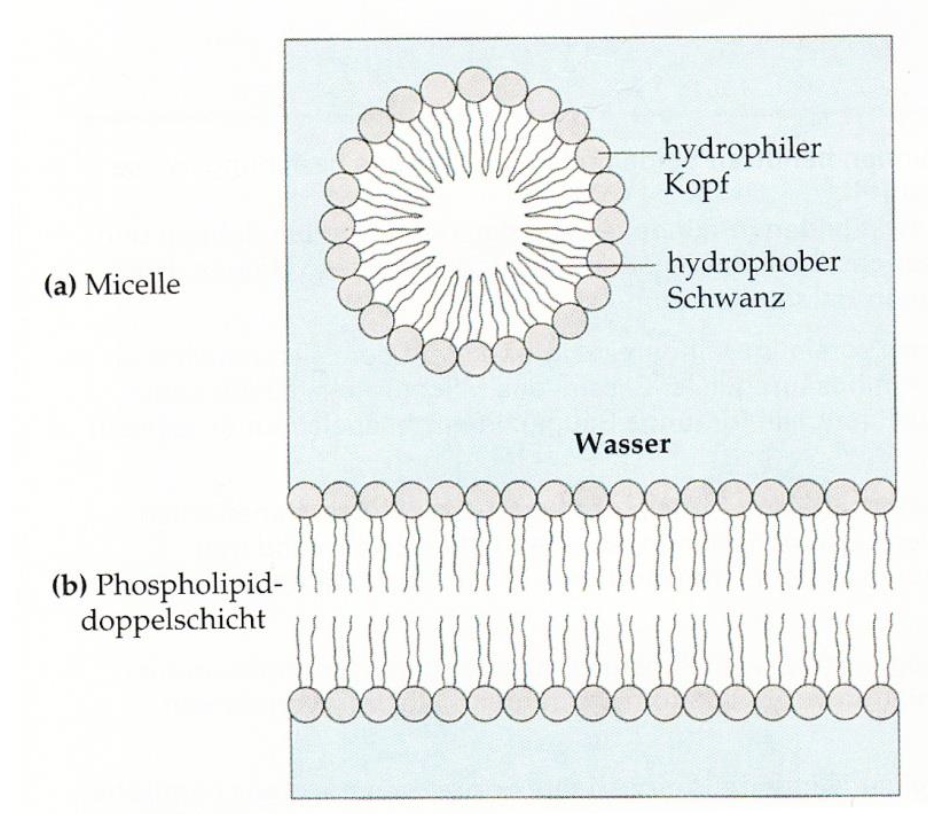
\includegraphics[width=5cm]{lec6/figures/phospholipid.png}
    \hfill
    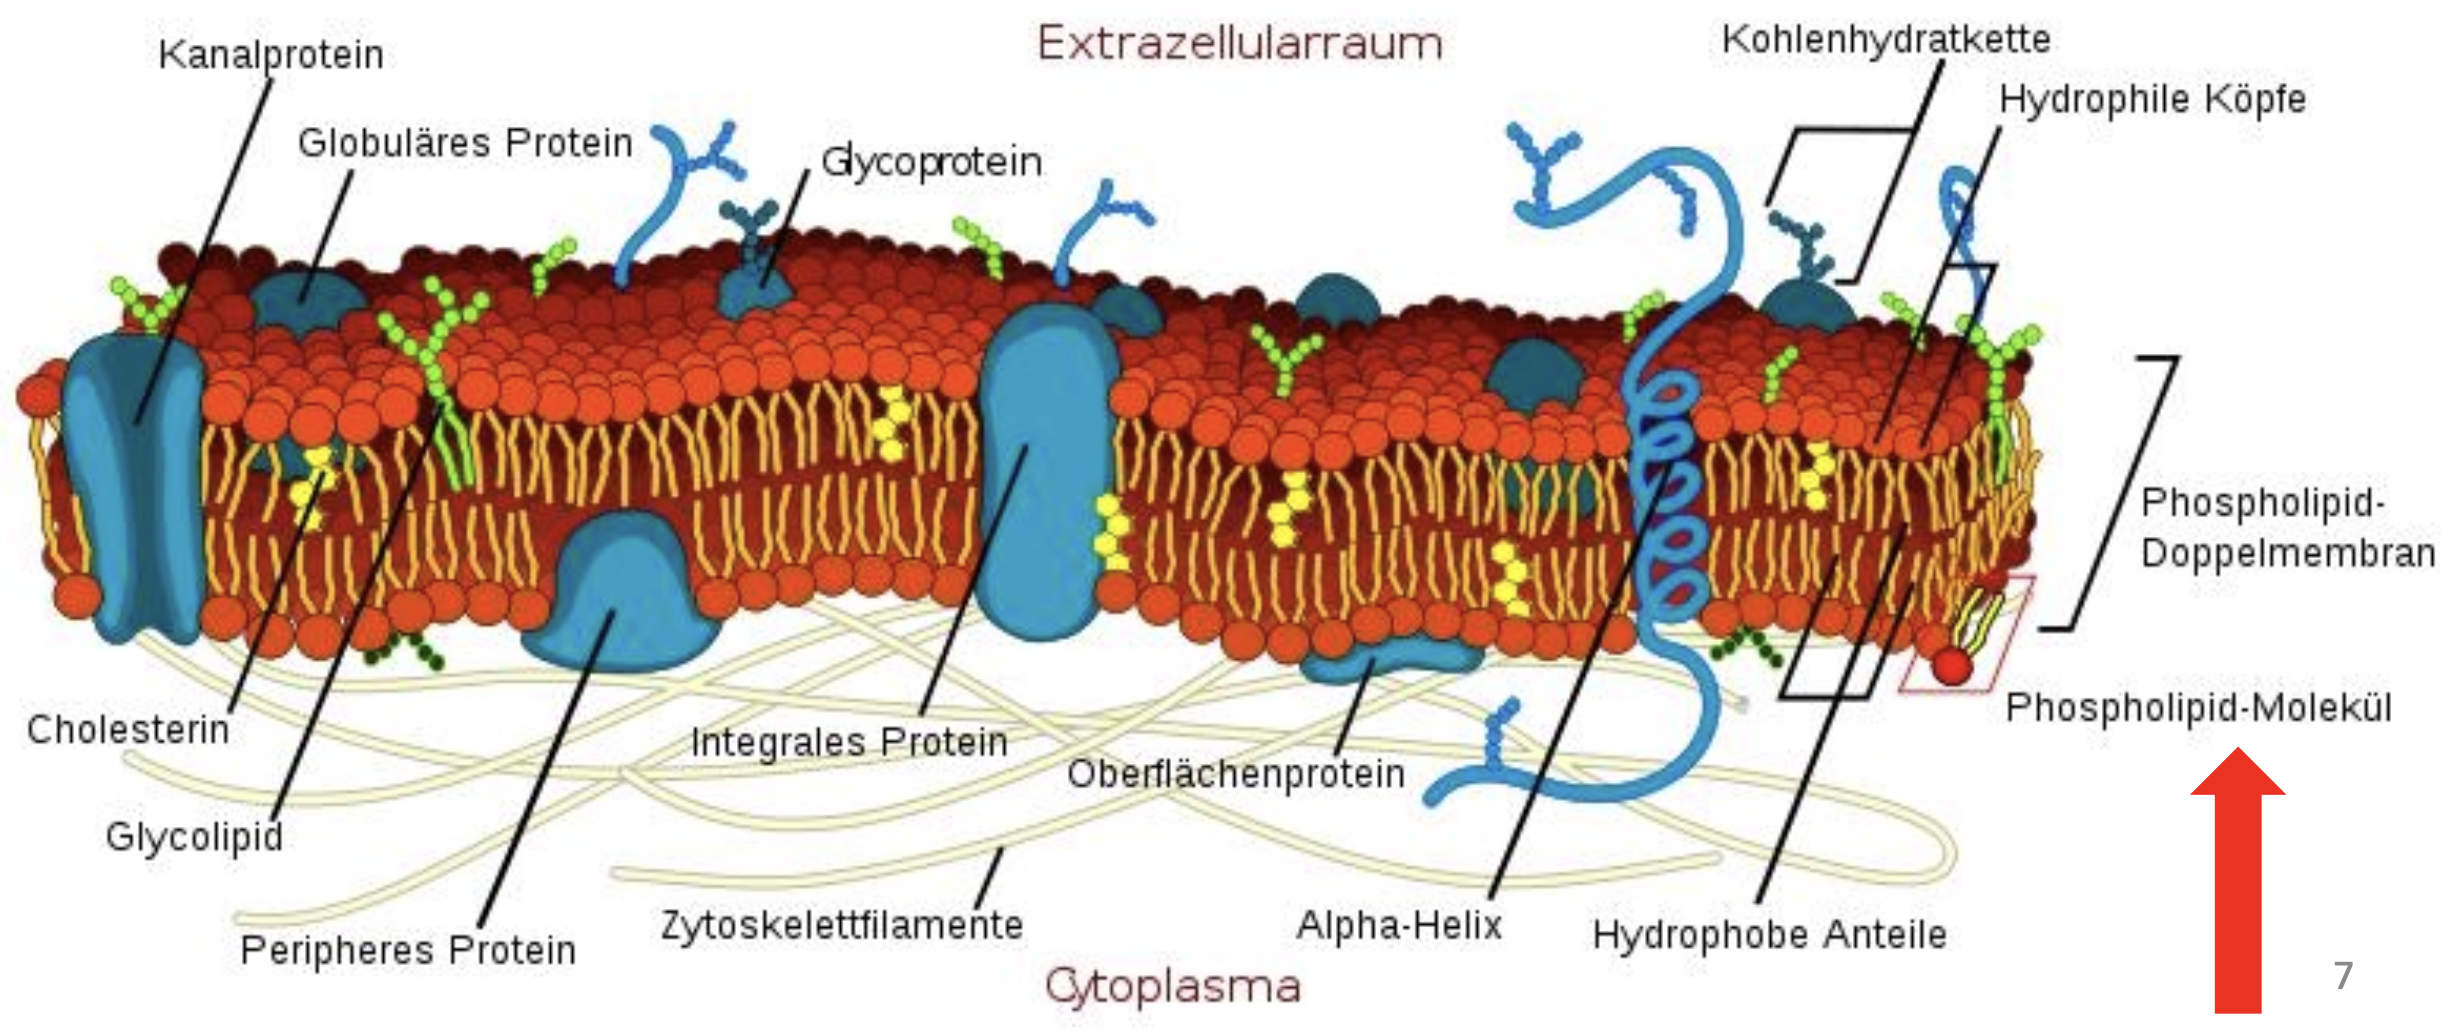
\includegraphics[width=10cm]{lec6/figures/zellwand.png}
\end{center}
\textbf{Bspl.\ Schwarmverhalten} von Vögeln/Fischen. Dient dem Schutz vor Jägern.
\\\\
\textbf{Bspl.\ Ameisenalgorithmus:} Wie wird der kürzeste Weg zwischen Nest (N) und Futterquelle (F) gefunden? Späherameisen finden Futterquellen zu Beginn auf zufälligen Wegen und hinterlassen dabei eine Pheromonspur. Weitere Ameisen folgen den Spuren zum Futter und hinterlassen selbst Pheromone. Da die Pheromone mit der Zeit verdunsten sind die Pheromonspuren auf kürzeren Spuren stärker als auf Längeren (da pro Zeit mehr Ameisen strömen) $\rightarrow$ Lösung wird optimiert ist aber nicht optimal. Nachteil: die optimale Lösung wird nie gefunden, wenn die Späherameisen nicht per Zufall auf sie stoßen. (Aus dem Internet: Ein Vorteil ist, dass als heuristischer Algorithmus schneller eine gute Lösung gefunden wird, als z.B.\ mit Breitensuche.)\\
\textit{Technische Anwendung:} Routing von Internetpaketen, Logistik, etc.
\\\\
(\dangersign \textit{Beschreibe den Ameisenalgorithmus + seine Vor- \& Nachteile.})
\\\\
\textbf{Bpsl.\ Schleimpilze (auf Zell-/Zellverbandebene):} Können sich in Verbänden fortbewegen + in schlechten Umgebungsbedingungen bildet sich durch Selbstorganisation ein ``Fruchtkörper'', der Sporen freisetzt. \textit{Technische Anwendung:} Schleimpilz wurde zu Beginn des Experimentes auf einer Oberfläche in Form der japanischen Küste ``in Tokio plaziert''. Andere Städte wurden mit Nahrung markiert. Zu Beginn wächst der Pilz auf vielen Wegen in alle Richtungen und löscht nach einiger Zeit ``ineffiziente Wege''. Es zeigt sich, dass das Verbindungsnetz des Schleimpilzes dem Bahn-Netz von Tokio ähnelt.
\\\\
(\dangersign \textit{Nenne Beispiele für Selbstorganisation.})
\\\\
(\dangersign \textit{Welcher einfache Organismus kann eine kürzeste Wegsuche durchführen wie die Ameisen?})

\begin{center}
    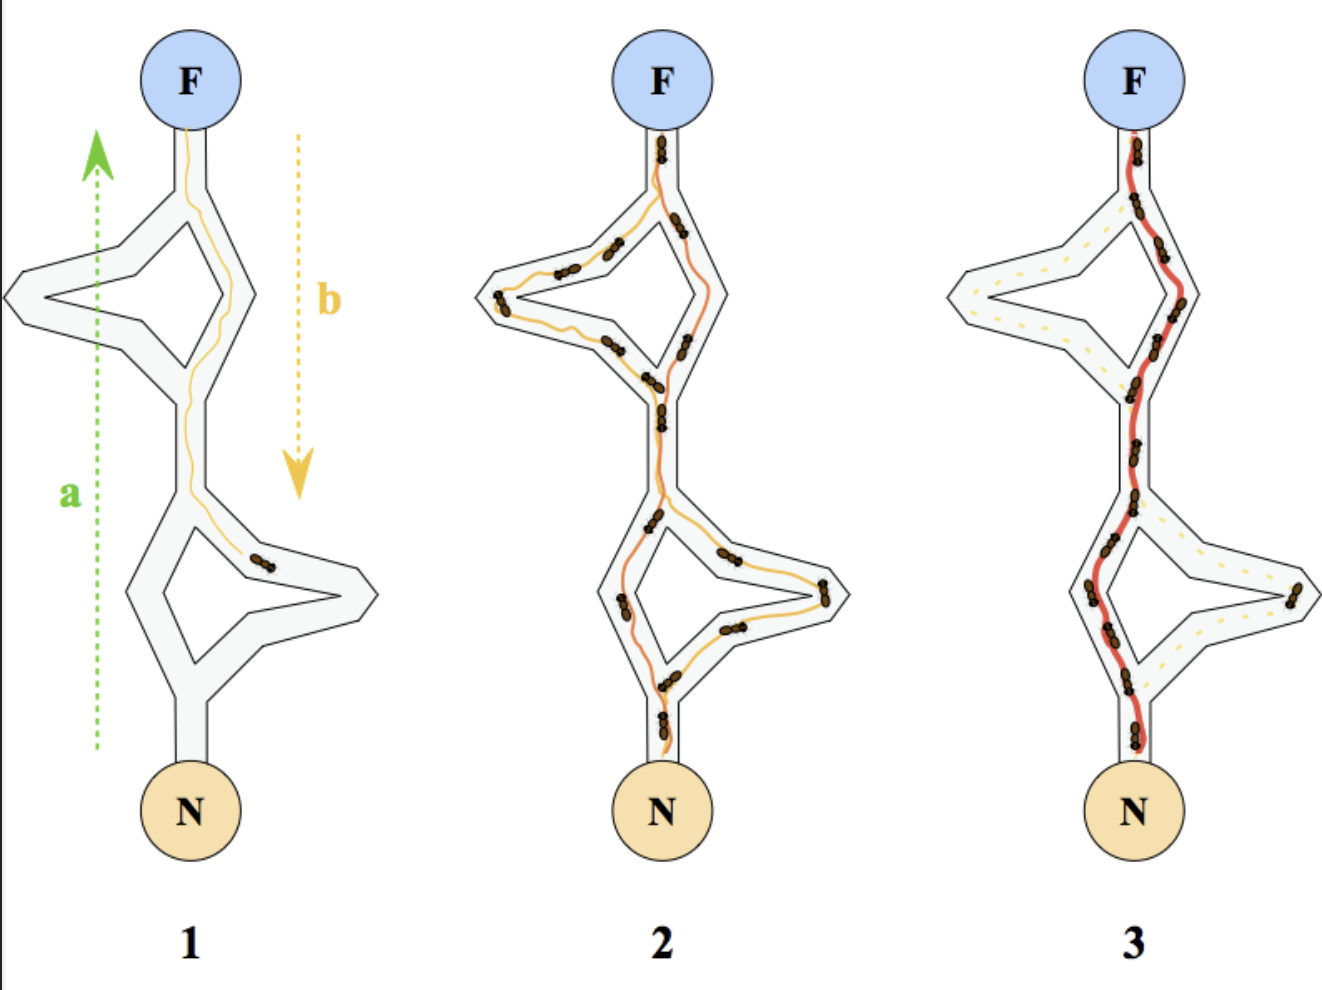
\includegraphics[width=6cm]{lec6/figures/ameisenalg.png}
    \hfill
    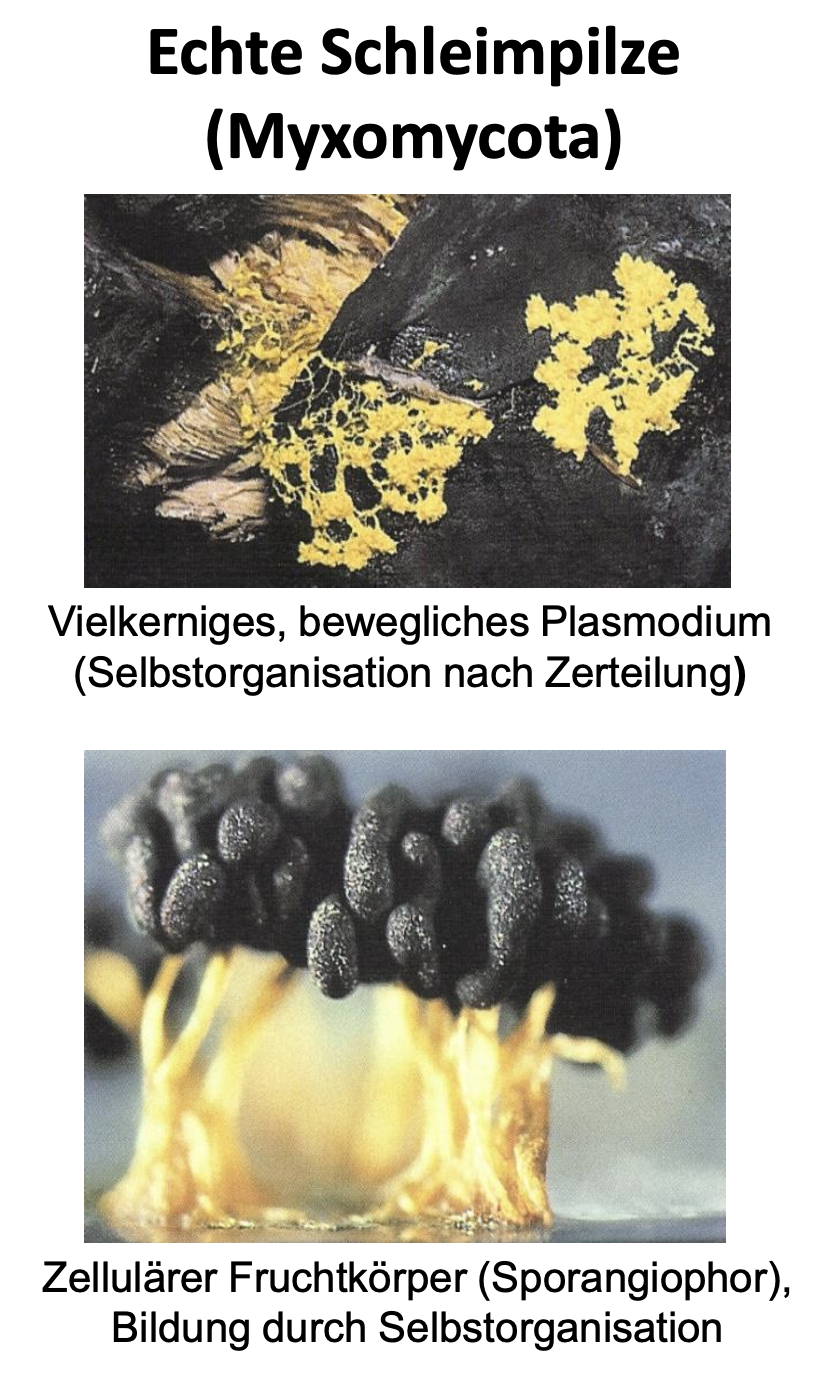
\includegraphics[width=4cm]{lec6/figures/schleimpilz.png}
    \hfill
    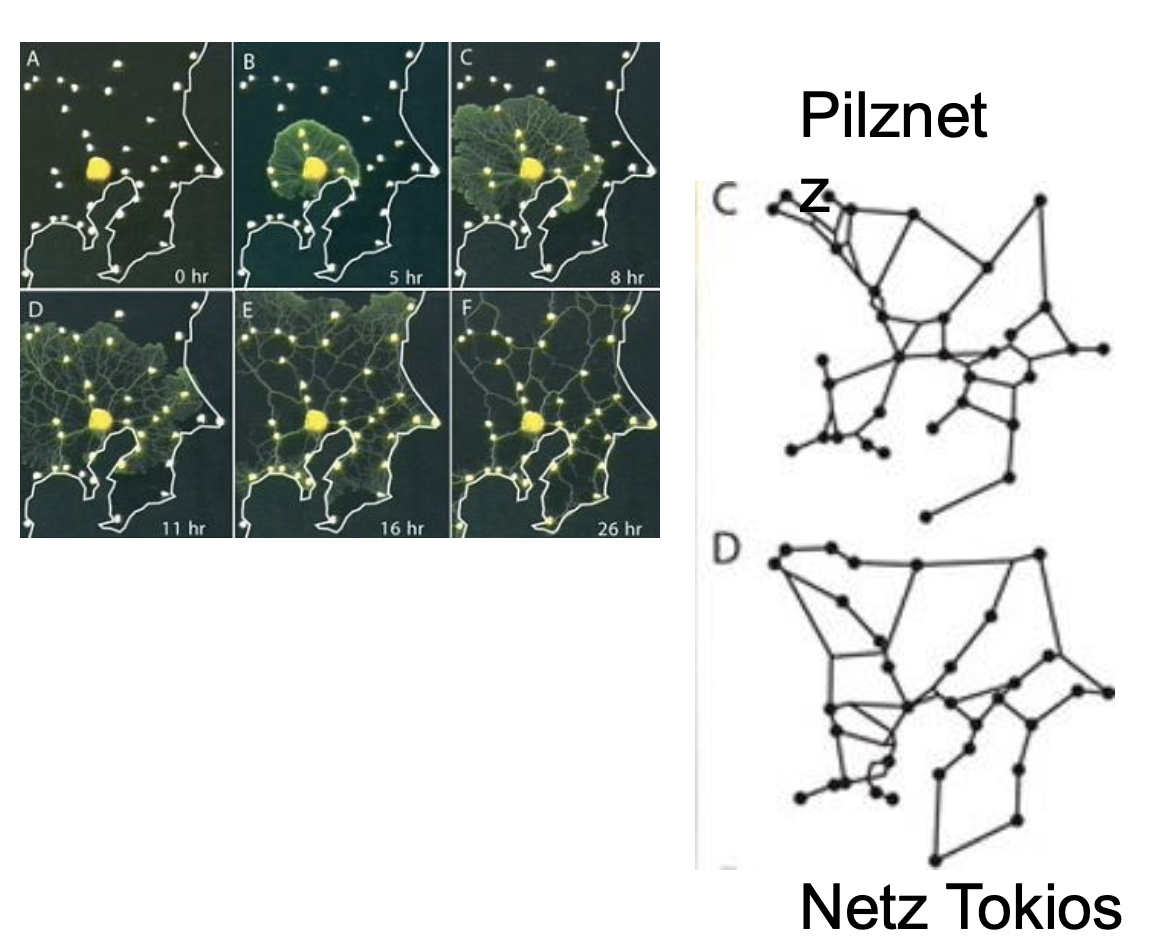
\includegraphics[width=6cm]{lec6/figures/japan.png}
\end{center}
\textbf{Bspl.\ der Selbstorganisation von komplexen Organismen: Glasschwamm \& Rotbuche.} Der Glasschwamm ist in der Lage bei geringen Temperaturen Glaskristalle zu bilden und Glasfasern zu einem Gesamtskellett zu verweben. Im Verlauf der Entwicklungsstadien der Rotbuche organisiert sie sich vom Samen, zum Keimling und Baum.
\begin{center}
    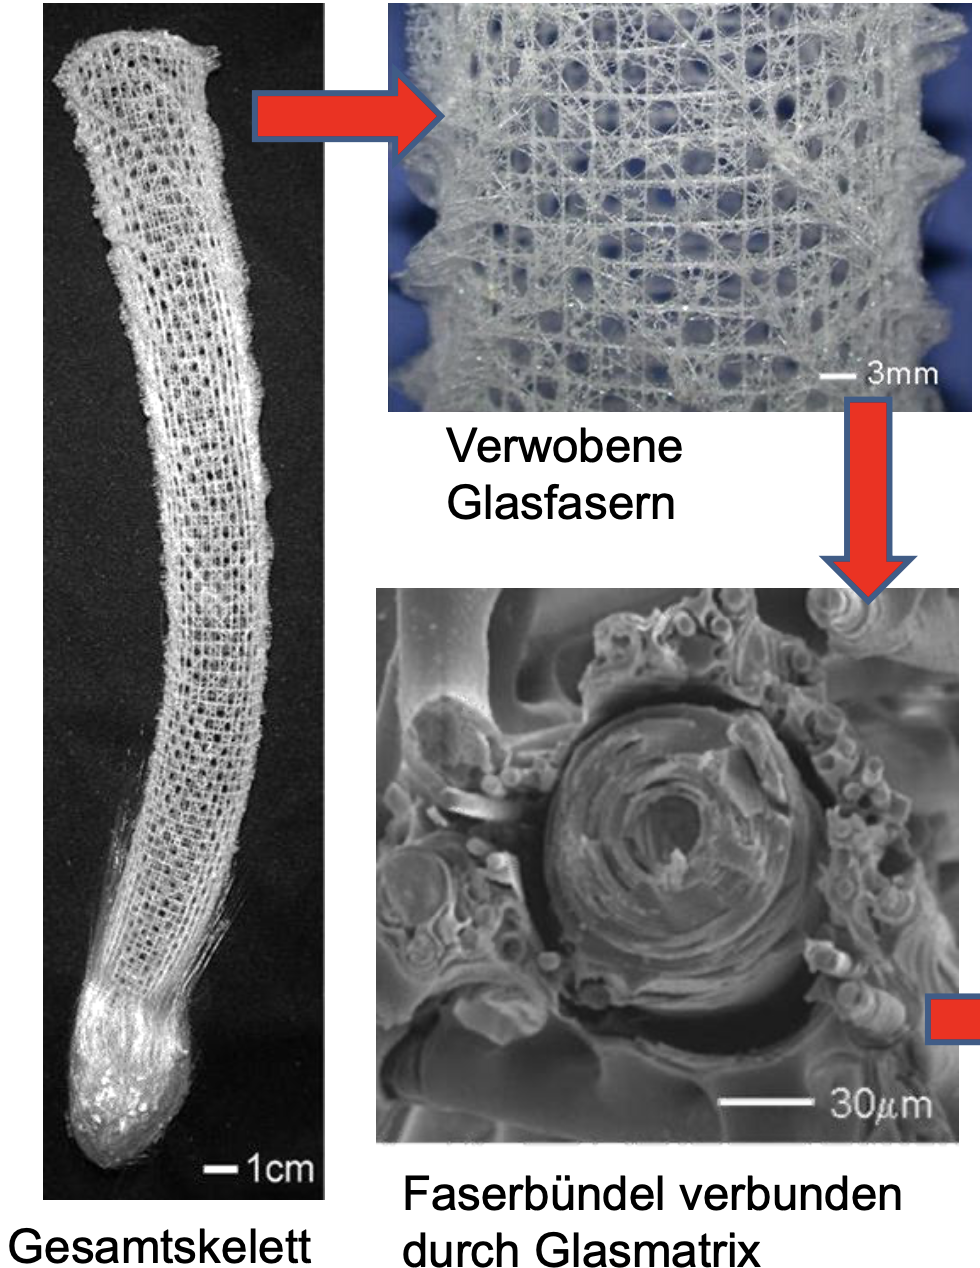
\includegraphics[width=4.5cm]{lec6/figures/Glasschwamm.png}
    \hfill
    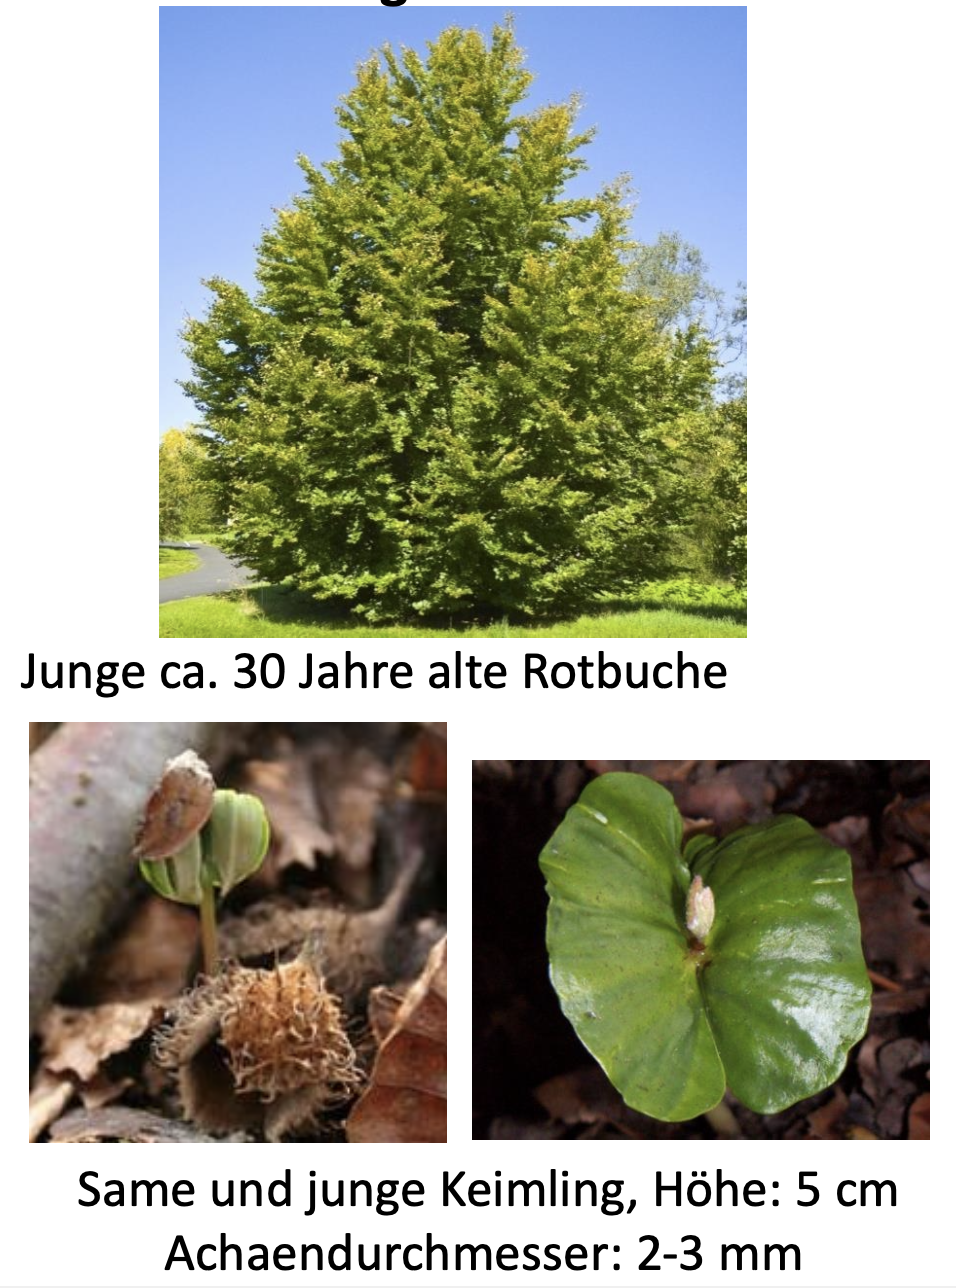
\includegraphics[width=5cm]{lec6/figures/Rotbuche.png}
\end{center}
Biologische Strukturen
\begin{itemize}
    \item sind anpassungsfähig an variable Umweltbedingungen,
    \item haben einer hohe Schadenstoleranz + Selbstreparaturvermögen und
    \item unterliegen den evolutionären Randbedingungen (z.B.\ die Federn des Pfaus diesen reproduktiven Zwecken).
\end{itemize}

\subsection{Pflanzliche Festigungsgewebe: Holz}

Jahresringe entstehen durch zyklische Änderungen des Umgebungsklimas. Bäume sind adaptive, multifunktionale Strukturen (\dangersign \textit{Welche besonderen Funktionen machen Bäume für
die Bionik so interessant}):
\begin{itemize}
    \item Mechanik (Holz): Biege- und Torsionssteifigkeit, Zähigkeit, Schwingungsdämpfung, Schadenstoleranz
    \item Transport (Holz \& Phloem): Transport von Wasser und Nährsalzen (stammaufwärts) von Assimilaten (stammabwärts)
    \item Speicherung (Holz \& Phloem): Nährstoffe und Wasser
    \item \textcolor{red}{Mechanischer Schutz, Schutz vor Pilzen \& Frass, Hitzeisolation (Borke \& Rinde): Schutz vor Waldbränden}
    \item Ernährung (Rinde, bei einigen Arten): Photosynthese Adaptives Wachstum (Holz): Bildung von Reaktionsholz
    \item Selbstreparatur: Reparatur von Rissen und Wunden hervorgerufen durch Verletzungen, überkritischen Belastungen, und/oder Wachstumsprozessen (Kambium, Parenchym)
\end{itemize}
\textit{In der folgenden Abbildung wurde auf Borke, Bast, Kambium und Jahrring eingegangen.}
\begin{center}
    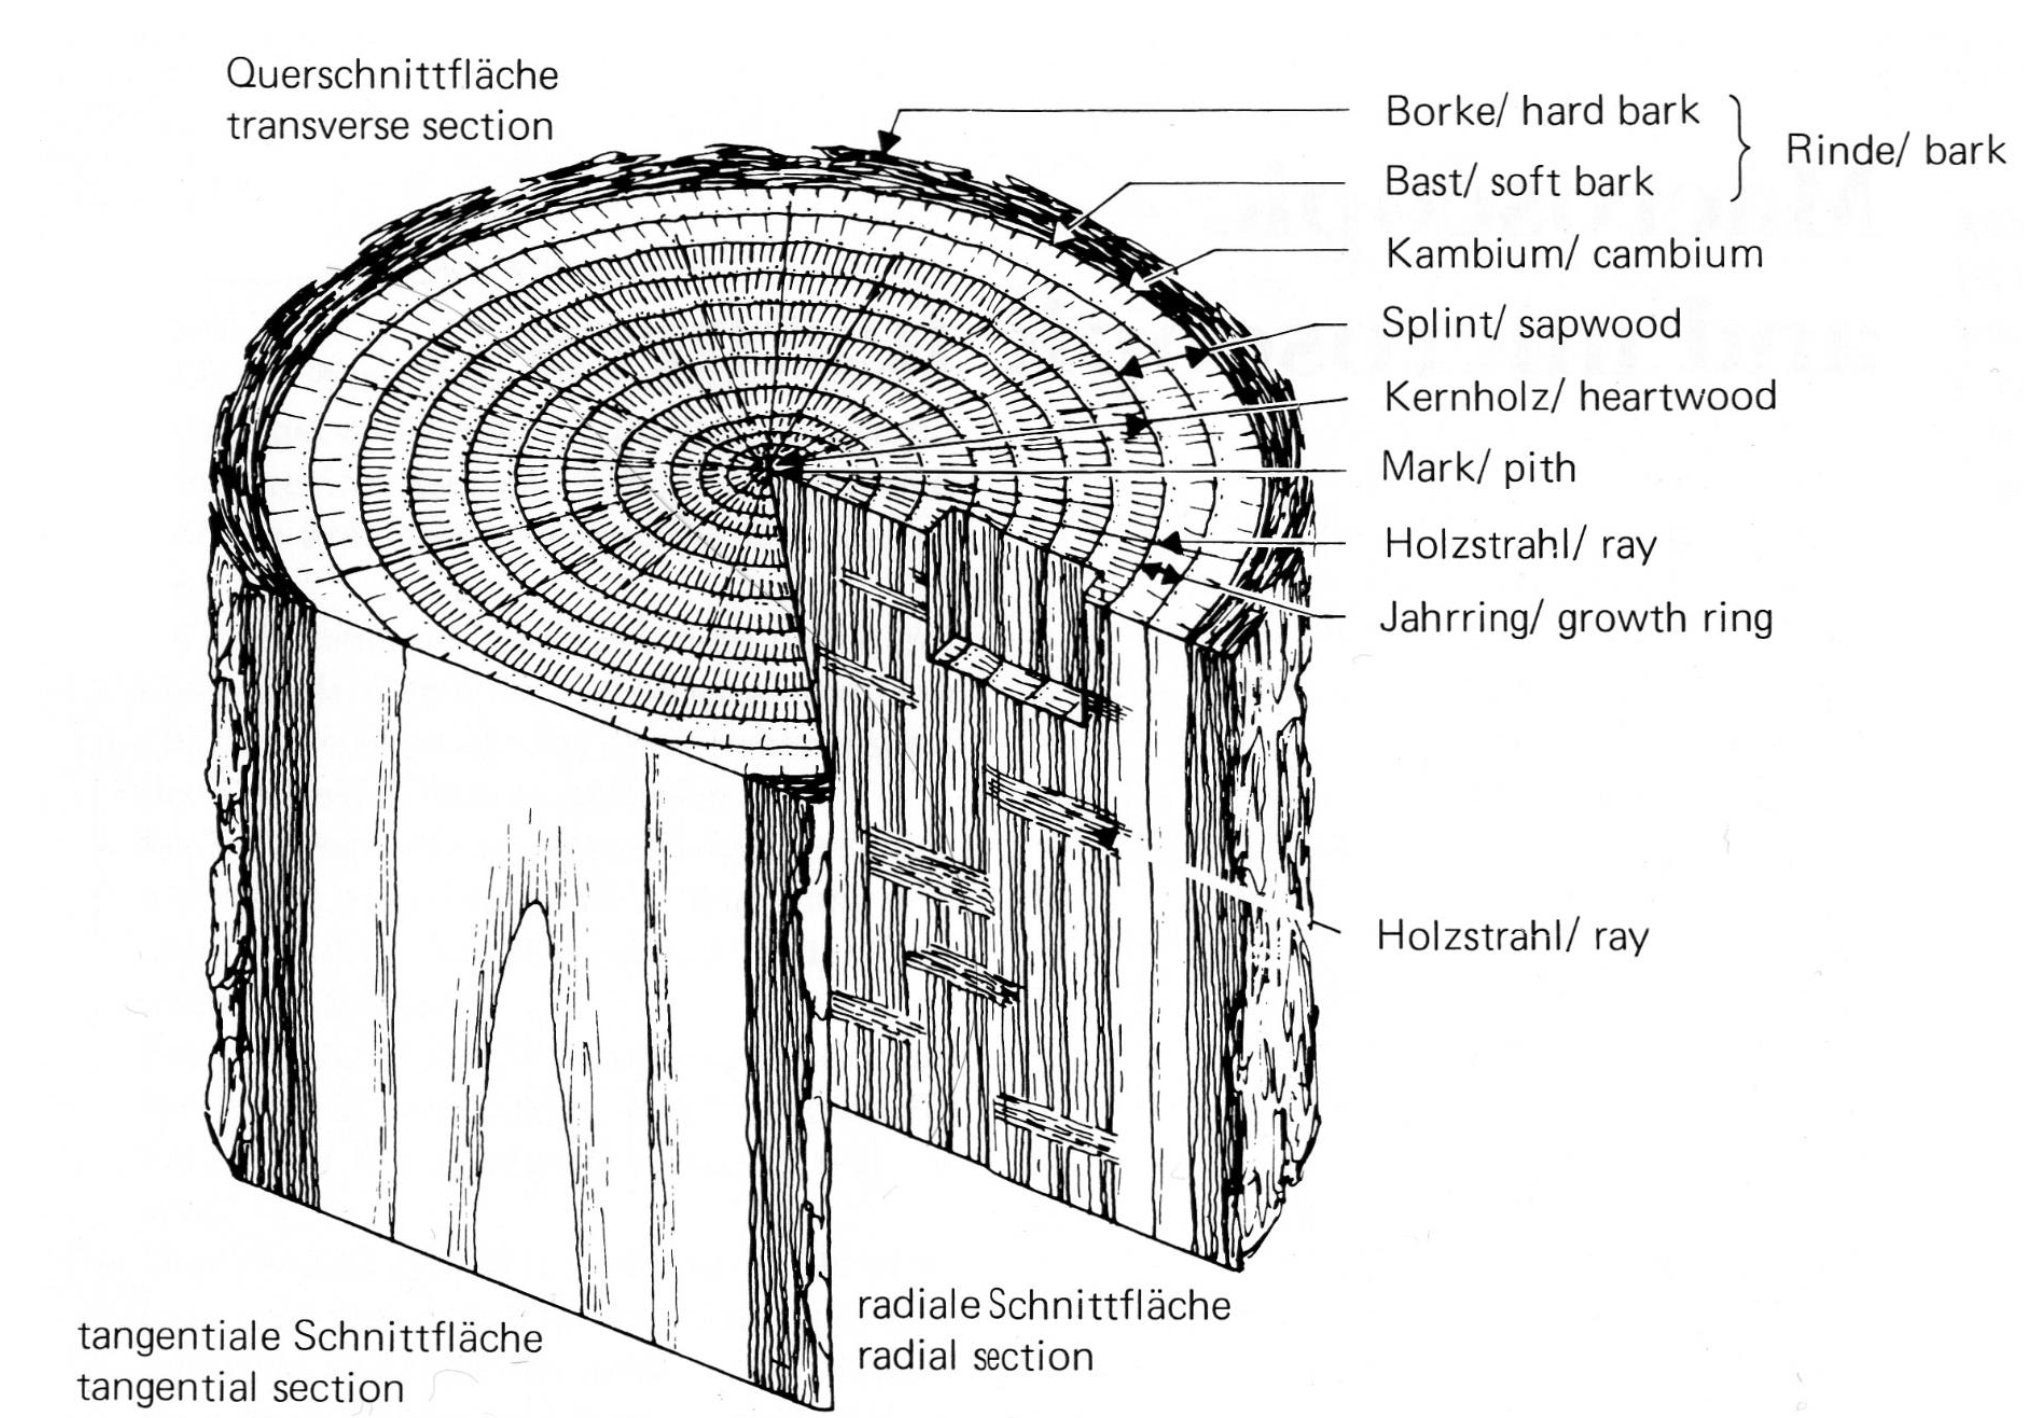
\includegraphics[width=7cm]{lec6/figures/holz.png}
\end{center}

\subsection{Bionische Verpackungen}

\subsubsection{Rinde von Bäumen als Hitzeisolation}

Während ``kalte'' Oberflächenfeuer häufig eine positive Wirkung für Pflanzen haben beschädigen Grund- und Kronenfeuer die Bäume. \textcolor{red}{Gemessen wird die Waldbrandanpassung eines Baumes an der Zeit $\tau_{60}$} nach der 60°C am Kambium erreicht sind \dangersign (Letaltemperatur für das lebende Kambium). Im nachfolgenden Bild sind $\tau_{60}$ Zeiten auf Versuchen für verschiedene Bäume aufgetragen $\rightarrow$ die Rindendicke korreliert mit der $\tau_{60}$ Zeit \dangersign. Gleichzeitig haben Bäume in Gebieten mit häufigen Waldbränden eine geringe Rindendichte und hohen Strukturierungsgrad.

\begin{center}
    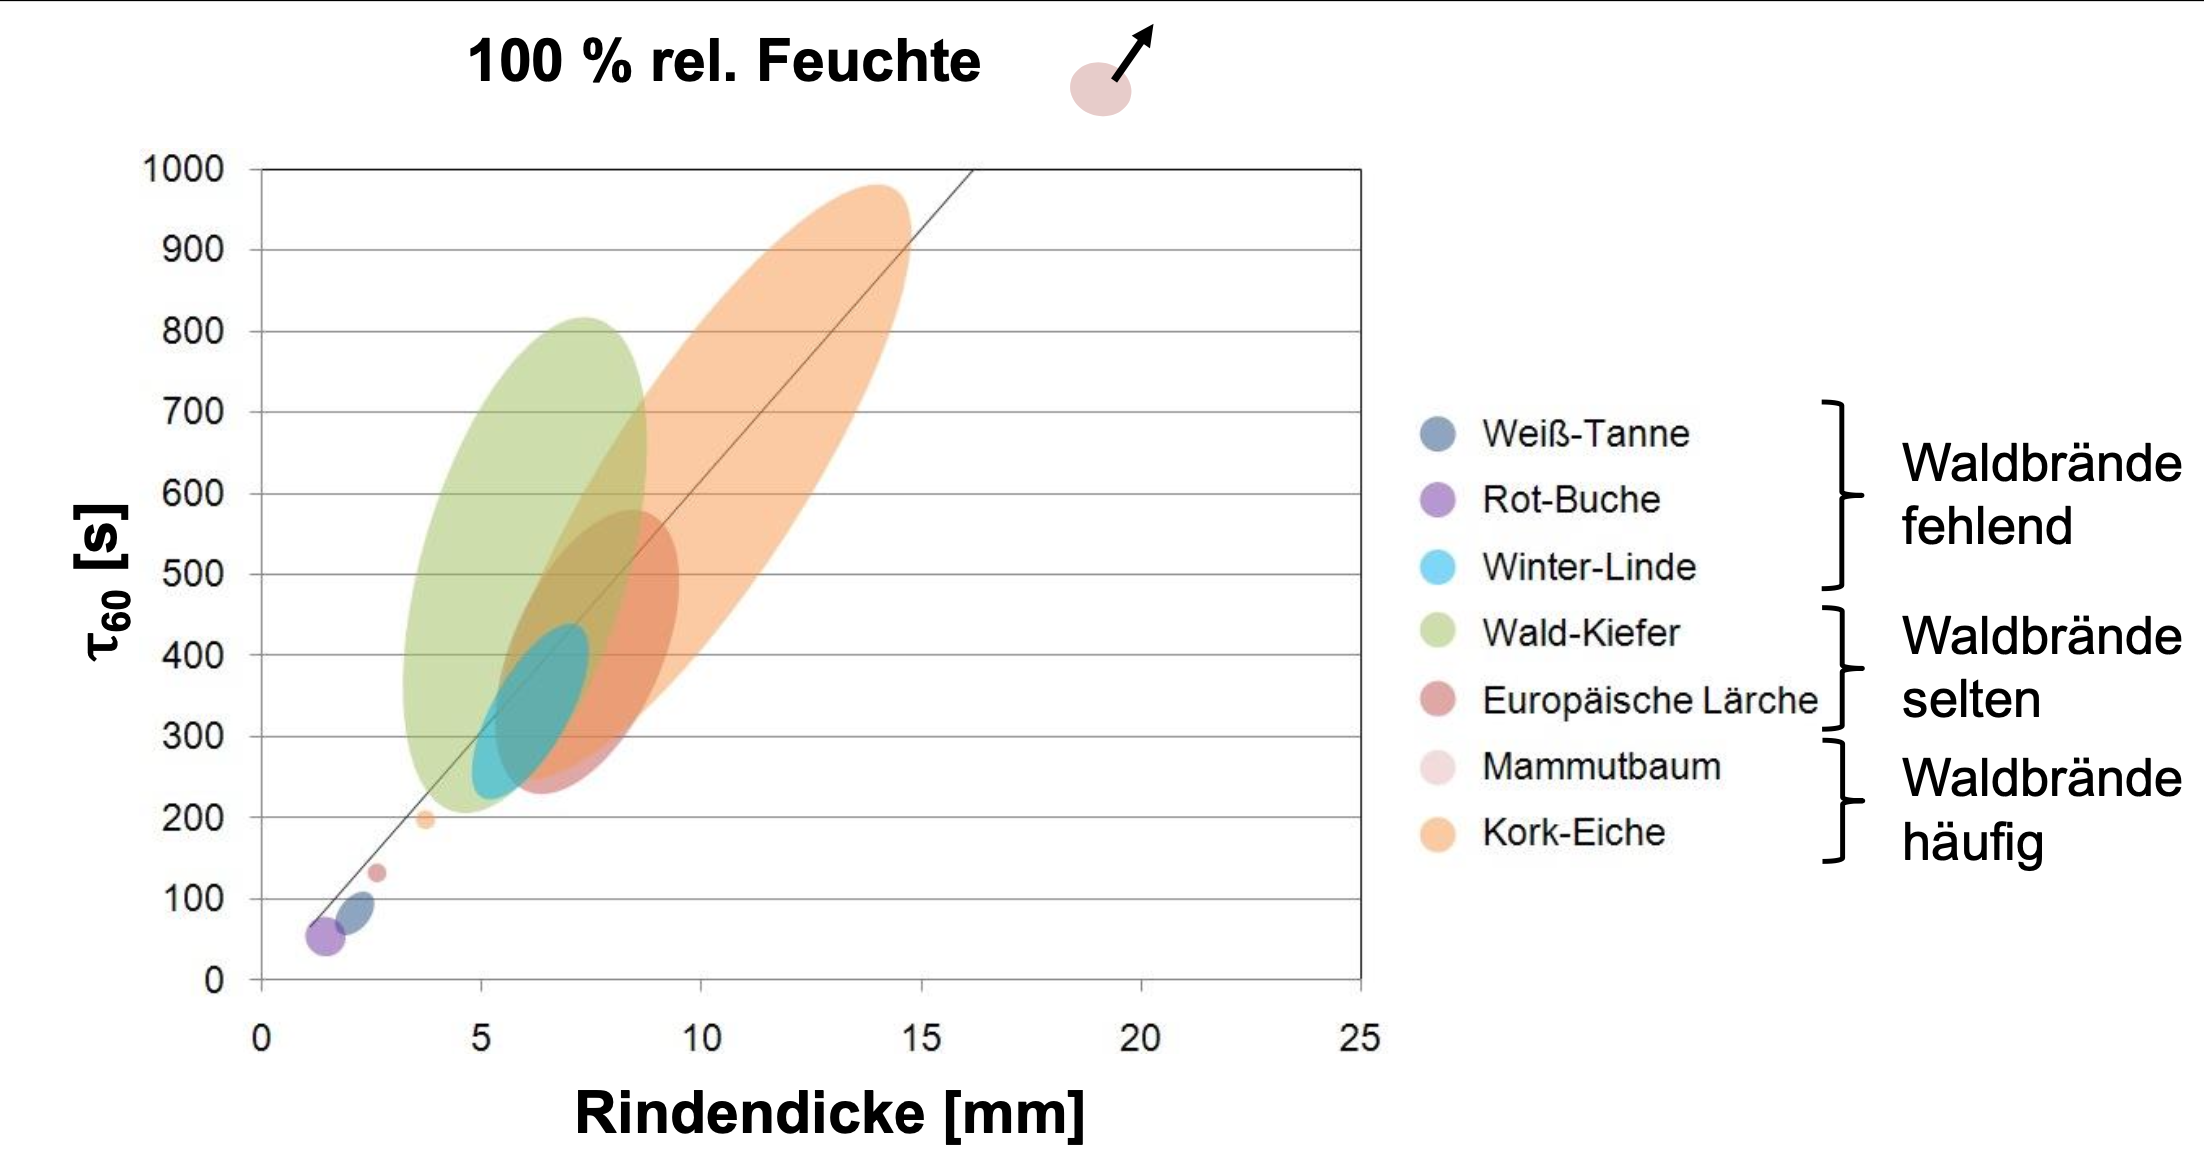
\includegraphics[width=8cm]{lec6/figures/rindendicke.png}
    \hfill
    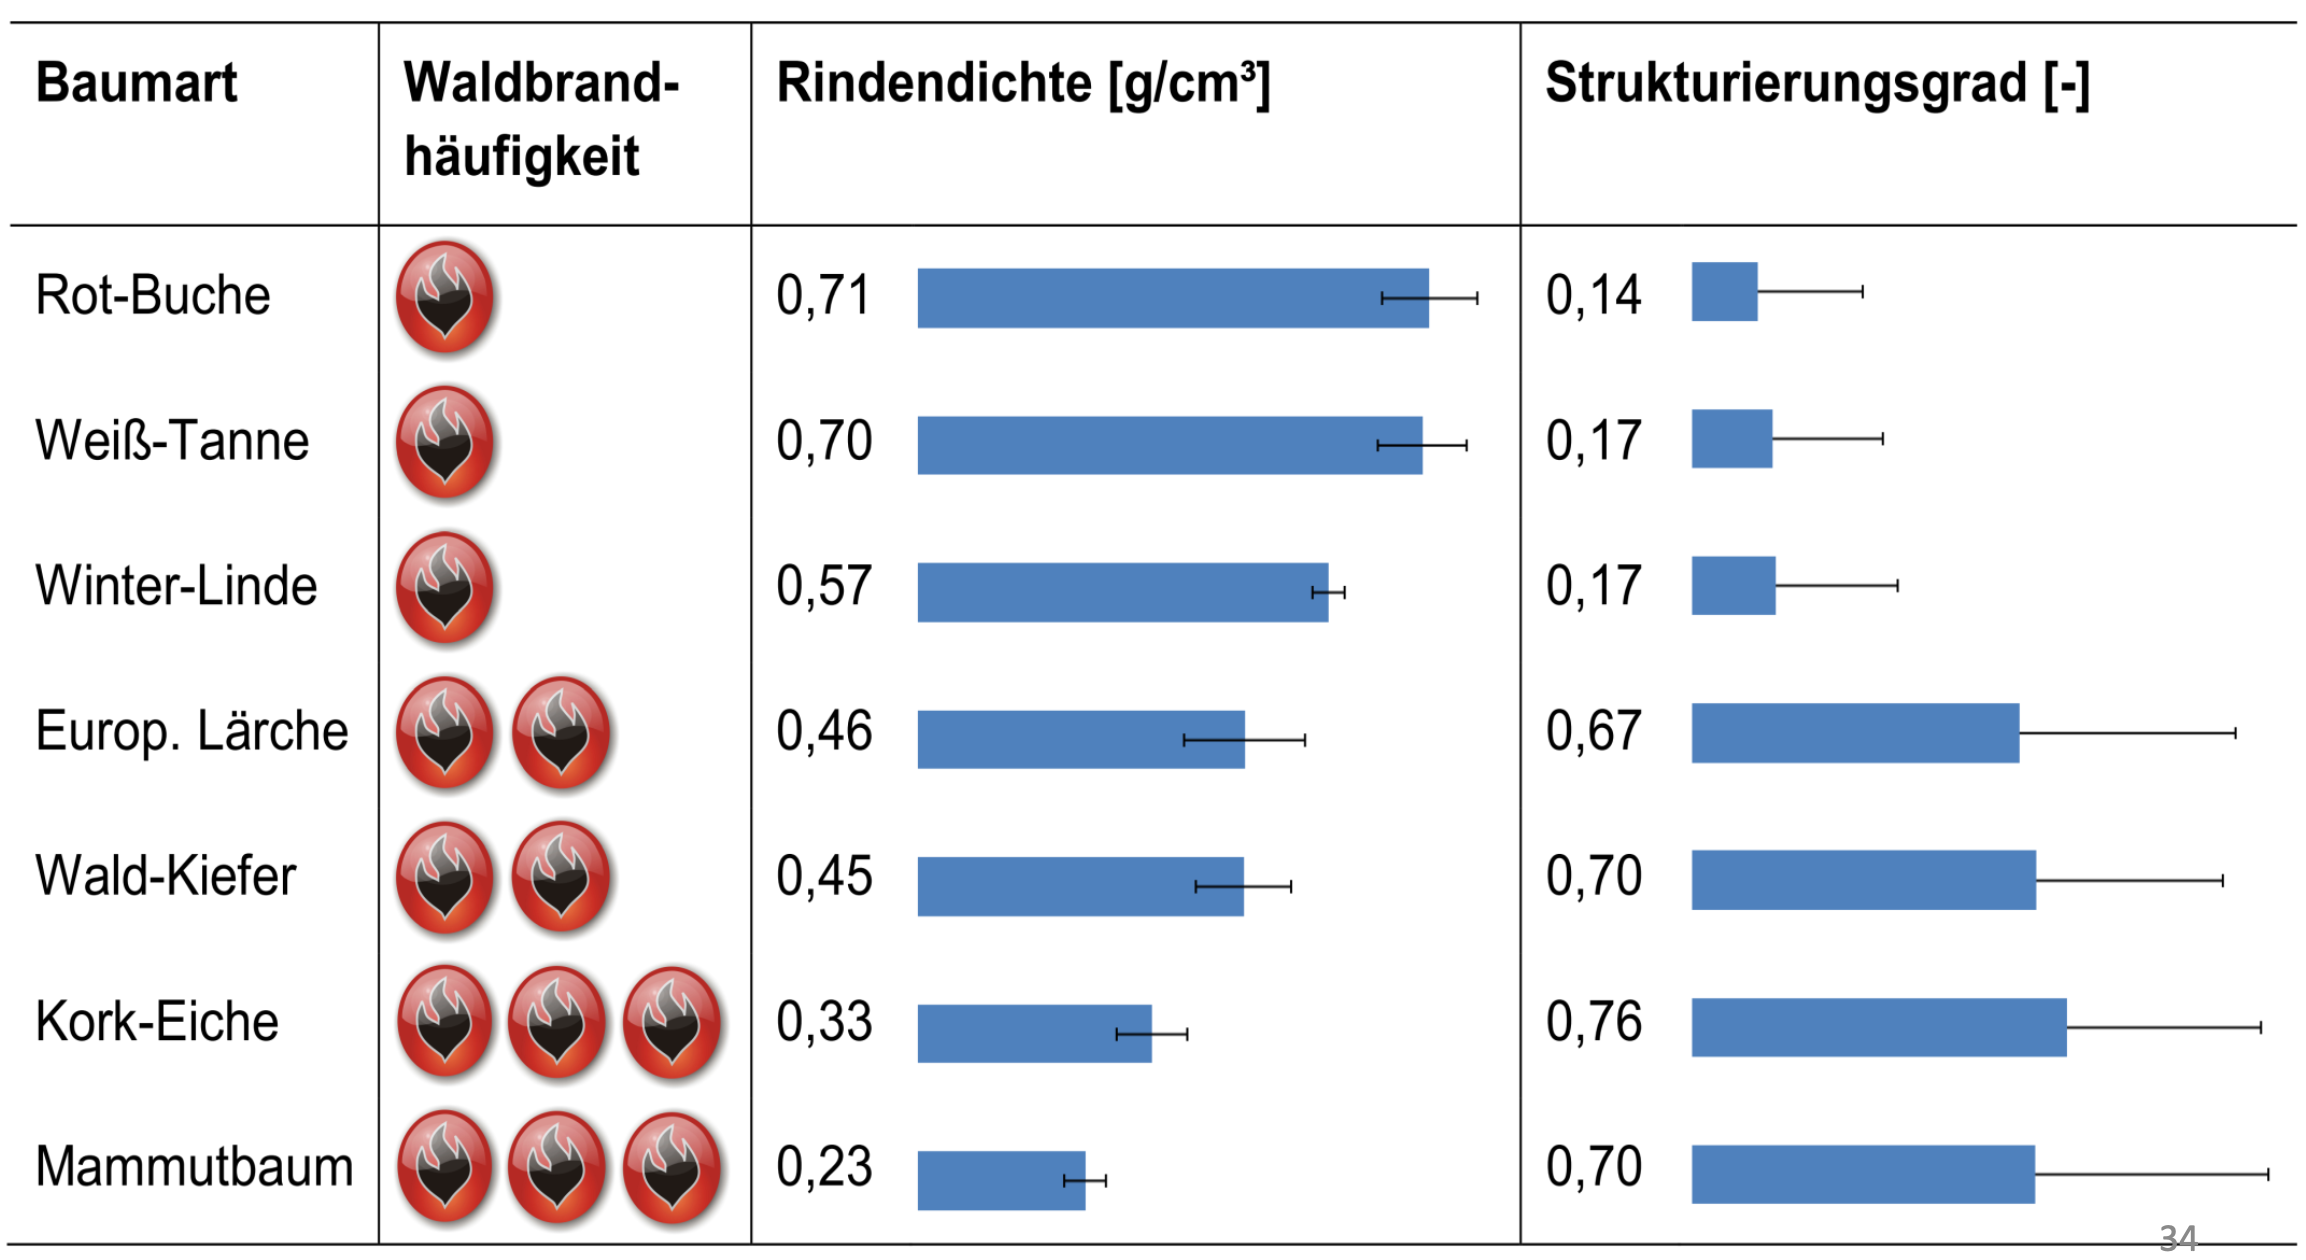
\includegraphics[width=8cm]{lec6/figures/rindendichte.png}
\end{center}
\textit{Technische Umsetzung:} Verwendung von biogenem Rindematerial, z.B.\ Korkplatten. \textit{Bionische Umsetzung:} Entwicklung bionisch-technischer Materialien anhand der physikalischen \& chemischen Rindeneigenschaften.

\subsubsection{Adaptive Strukturen in der Rinde fossiler Pflanzen für adaptive bionische Hüllen}

Fossile Pflanzenreste zeigen eine netzartige Kambiumstruktur, die gestaucht wird während der Baumstamm wächst und anschließend die äußerste Rindenschicht zerreist und abwirft. Dabei muss das netzartige Kambium eine hohe Energie aufnehmen und aushalten -- Ideengeber für die bionische Optimierung von adpativen Hüllstrukturen, z.B.\ Explosionsdämpfungssystemen (\dangersign $\rightarrow$ \textit{Bspl.}).

\begin{center}
    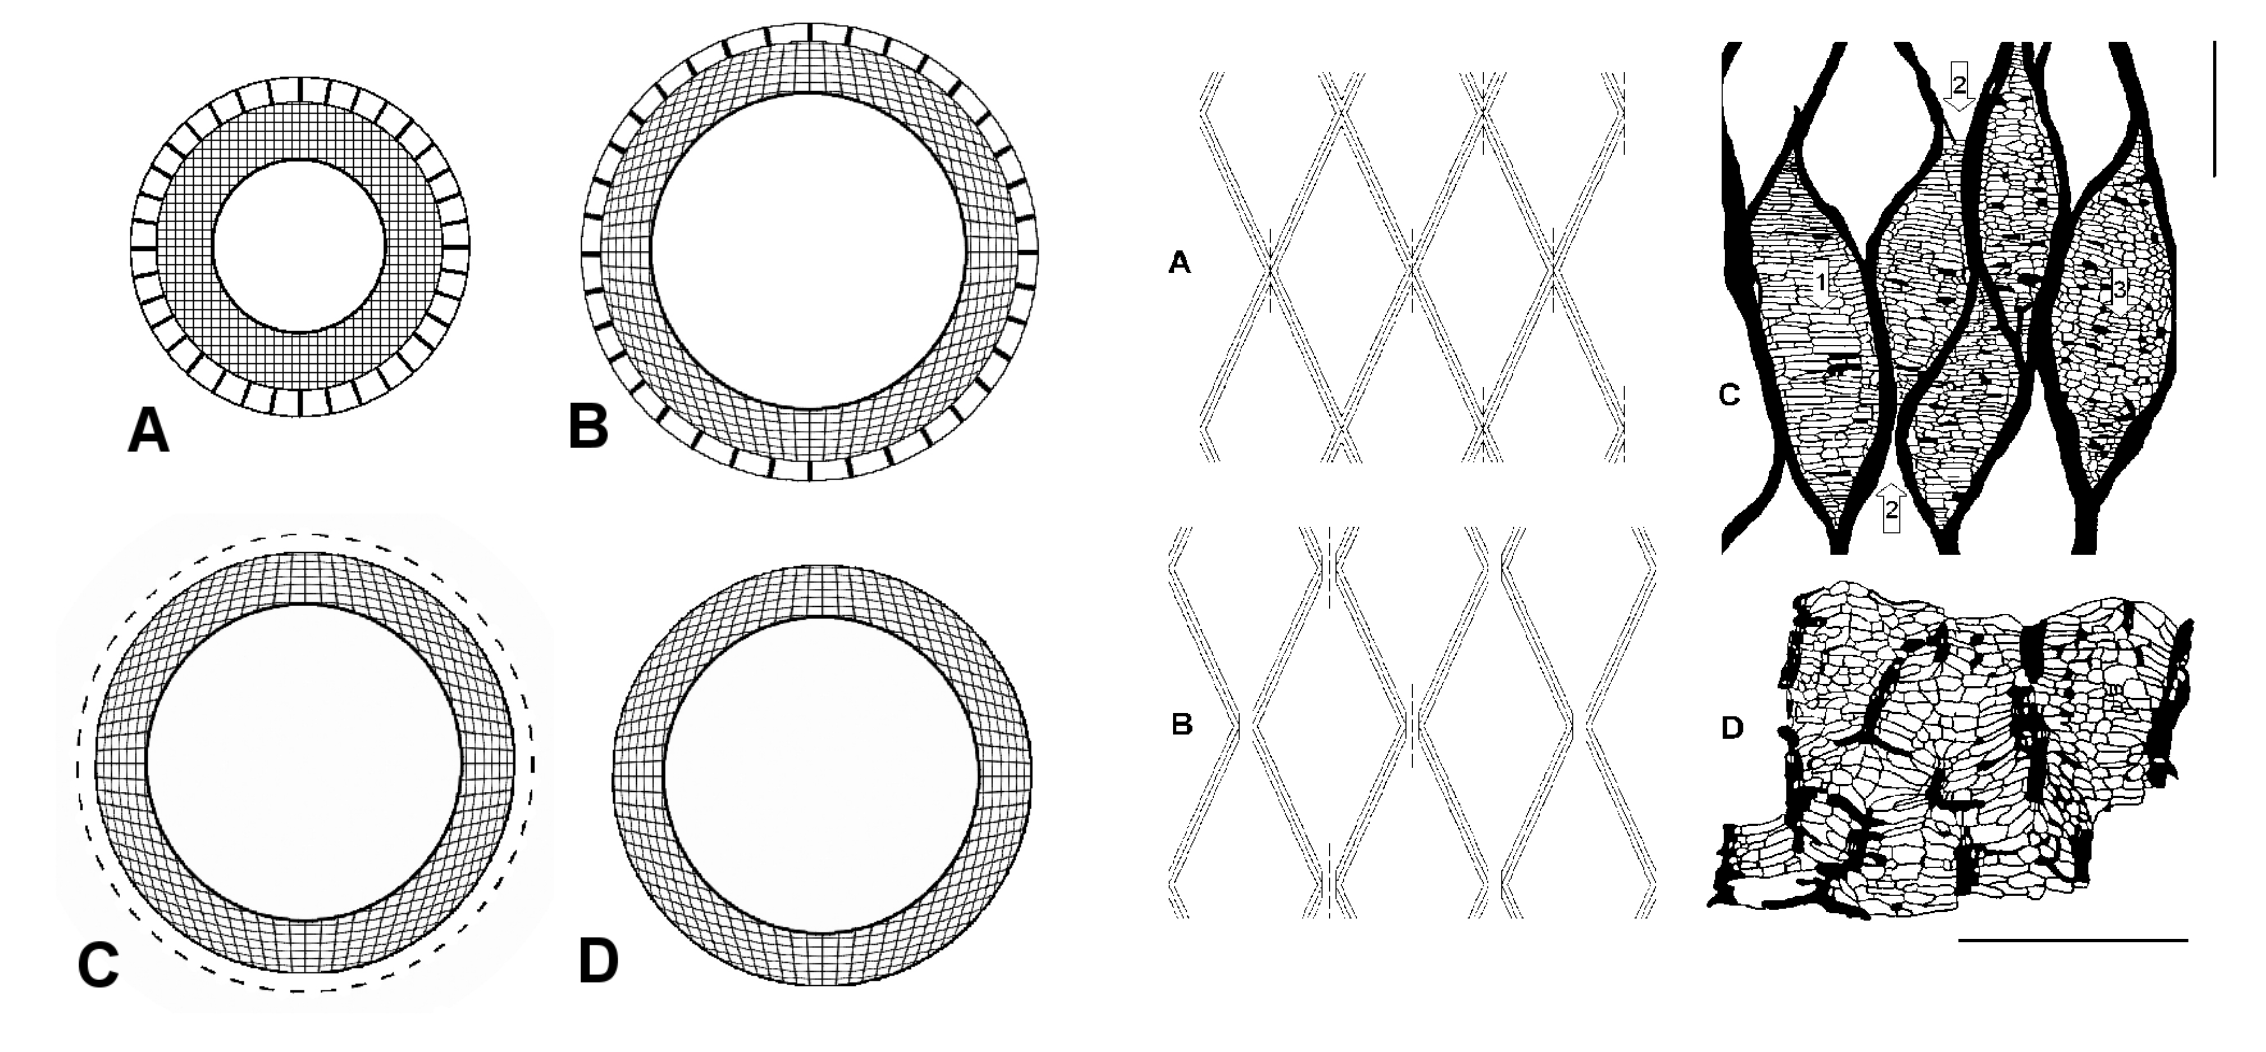
\includegraphics[width=8cm]{lec6/figures/rindennetz.png}
    \hfill
    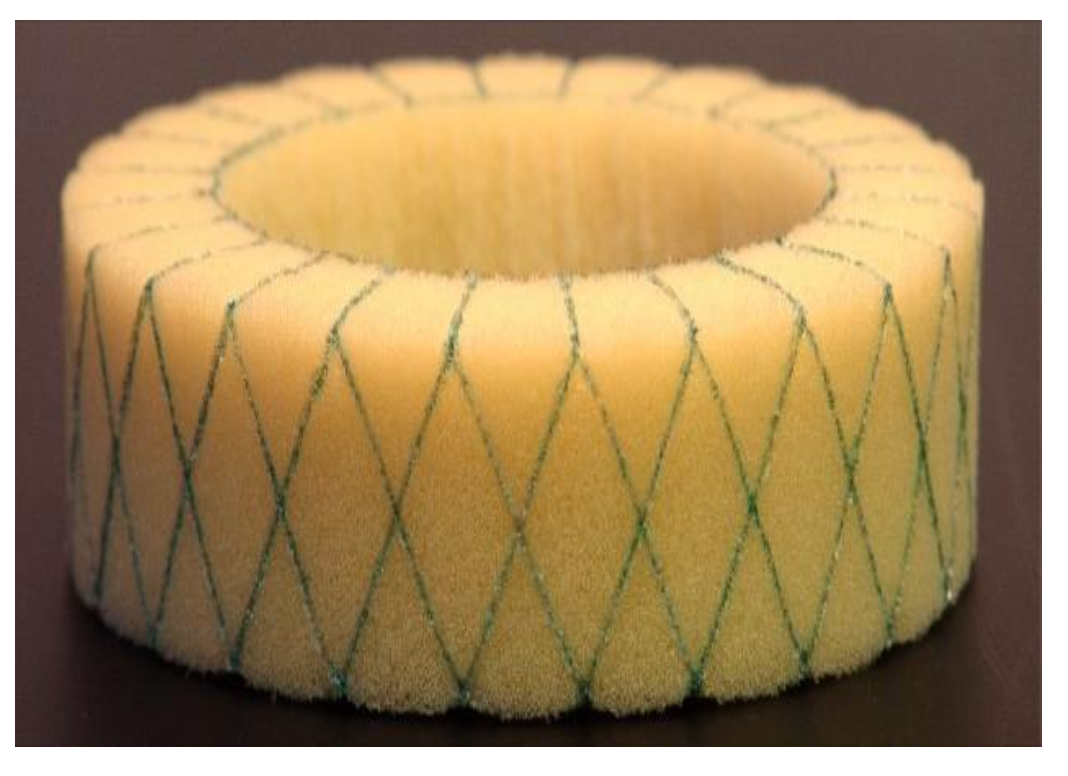
\includegraphics[width=4cm]{lec6/figures/explosion.png}
\end{center}

\subsubsection{Straußenei und Kokosnuss}

Interessante Eigenschaften vom \textbf{Straußenei}:
\begin{itemize}
    \item Hervorragende mechanische Eigenschaften (Druck- und Bruchstabilität), bedarfsgerechte Öffenbarkeit beim Schlüpfen des Kükens
    \item Material- und strukturoptimierte Eischale, die Gasaustausch ermöglicht
    \item Optimiertes Oberflächen-Volumen-Verhältnis
    \item Schutz des Inhaltes (Embryo \& Nährstoffe) gegen Hitze, UV-Strahlung, Bakterien- und Pilzbefall ...
    \item Langfristiger Schutz des verderblichen, lebendigen Inhalts
    \item Vollständige Rezyklierbarkeit der Eischale
\end{itemize}

\textit{Mögliche bionische Anwendung:} Atmungsaktive, bakterienresistente Frischhaltefolie. (\dangersign $\rightarrow$ \textit{Bspl.})
\\\\
Auch verschiedene Früchte bieten Ideen für bionische Verpackungen. Früchte werden nur von Blütenpflanzen gebildet und sind ``Blüten im Zustand der Samenreife''. Sie dienen dabei dem Schutz und der Verbreitung der Samen. Es gibt Streufrüchte (Samen werden zur Zeit der Fruchtreife freigegeben), Sammelfrüchte (entstehen aus einer Blüte mit vielen Fruchtblättern, die je eine eigenständige Frucht bilden) und Schließfrüchte (Samen bleiben bis zur Verbreitung von der Fruchtwand eingeschlossen).

\begin{figure}[!h]
  \centering
  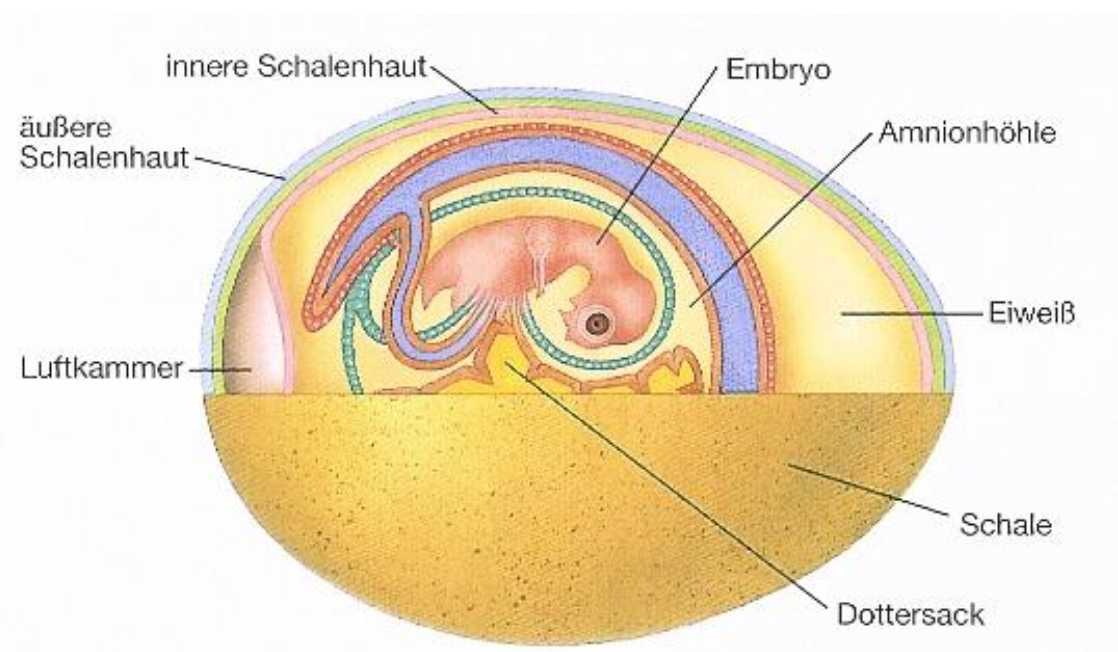
\includegraphics[width=8cm]{lec6/figures/ei.png}
  \hfill
  \begin{minipage}{.5\linewidth}
    \centering
      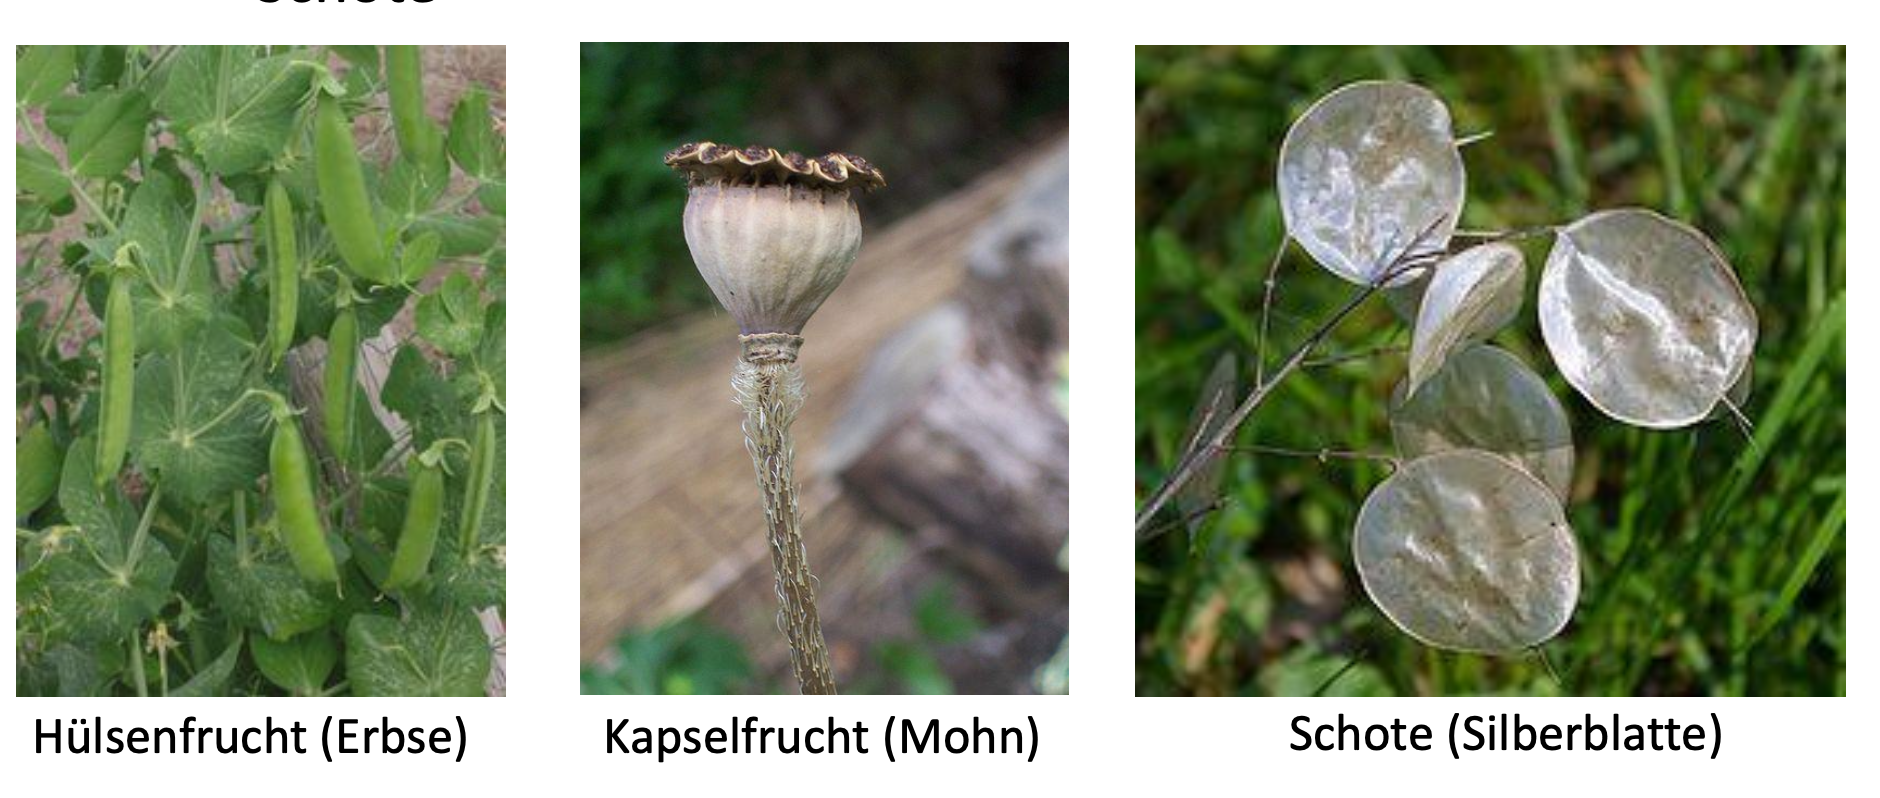
\includegraphics[width=\linewidth]{lec6/figures/streufrucht.png}
      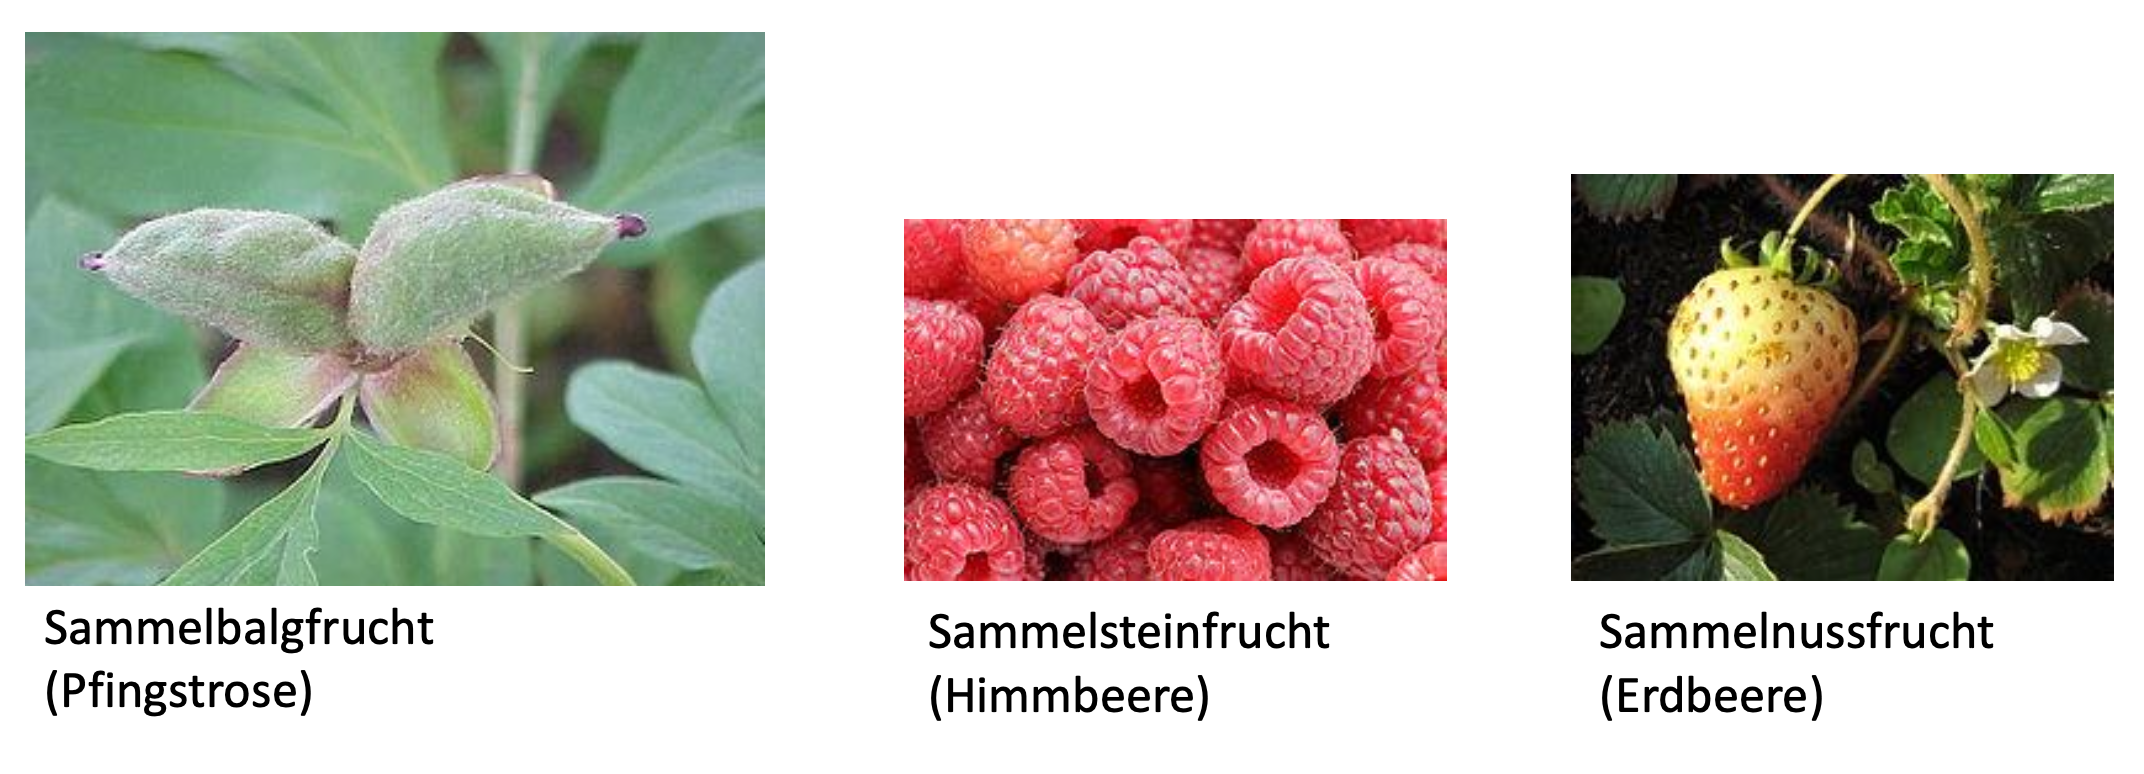
\includegraphics[width=\linewidth]{lec6/figures/sammelfrucht.png}
      \includegraphics[width=\linewidth]{lec6/figures/schließfrucht.png}
  \end{minipage}\quad
\end{figure}
Die \textbf{Kokosnuss} hat folgende für bionische Umsetzungen (\dangersign $\rightarrow$ \textit{Bspl.}) interessante Eigenschaften:

\begin{itemize}
    \item Hervorragende mechanische Eigenschaften (Dämpfung, Bruch- und Durchstoßstabiliät...) bedarfsgerechte Öffnung bei Keimung
    \item Optimiertes Oberflächen-Volumen-Verhältnis
    \item Schutz des Inhaltes (Keimling \& Nährstoffe) gegen Salzwasser, Hitze, UV-Strahlung, Bakterien- und Pilzbefall, Fressfeinde...)
    \item Monatelanger Transport in Salzwasser ohne Verlust der Keimfähigkeit, d.h. effektiver \& langfristiger Schutz des verderblichen Inhalts
    \item Vollständige Rezyklierbarkeit sämtlicher „Verpackungsmaterialien“
\end{itemize}

Bisher existieren keine bionischen Umsetzungen für Verpackungen anhand der Kokosnuss, obwohl diese die Vorraussetzungen für eine optimale Verpackung vom Deutschen Verpackungsinstitut und Bund Deutscher Verpackungsingenieure erfüllt. Aufgrung ihrer Zähigkeit, Härte und hoher Energiedissipation, eignet sich die Kokosnuss als Vorbild für Behälter für Gefahrengüter. Die Kokosnuss hat eine faserige Fruchtwand.
\\\\
Aufgrund der hohen Energiedissipation eignet sich die Fruchtwand der \textbf{Pomelo} für aufpralldämpfende und durchschlagsichere Helme. Die Pomelo hat eine sehr dicke, schaumartige Fruchtwand. In Aufpralltests aus dem freien Fall aus 6m wird über 90\% der \textbf{Energie dissipiert} $\rightarrow$ für aufpralldämpfende und durchschlagsichere Helme \hintsign.
\\\\
\textit{Technische Idee:} Hochbelastabares Material mit bionischer Schaum- und Faserstruktur (kompakte, teilweise faserverstärkte Aussenschicht + Metallschäume im Kern). (\dangersign $\rightarrow$ \textit{Bspl.})
\\\\
\textbf{Macadamia-Nuss:} Hohe Zähigkeit und Härte $\rightarrow$ schusssichere Westen \hintsign.

\begin{center}
    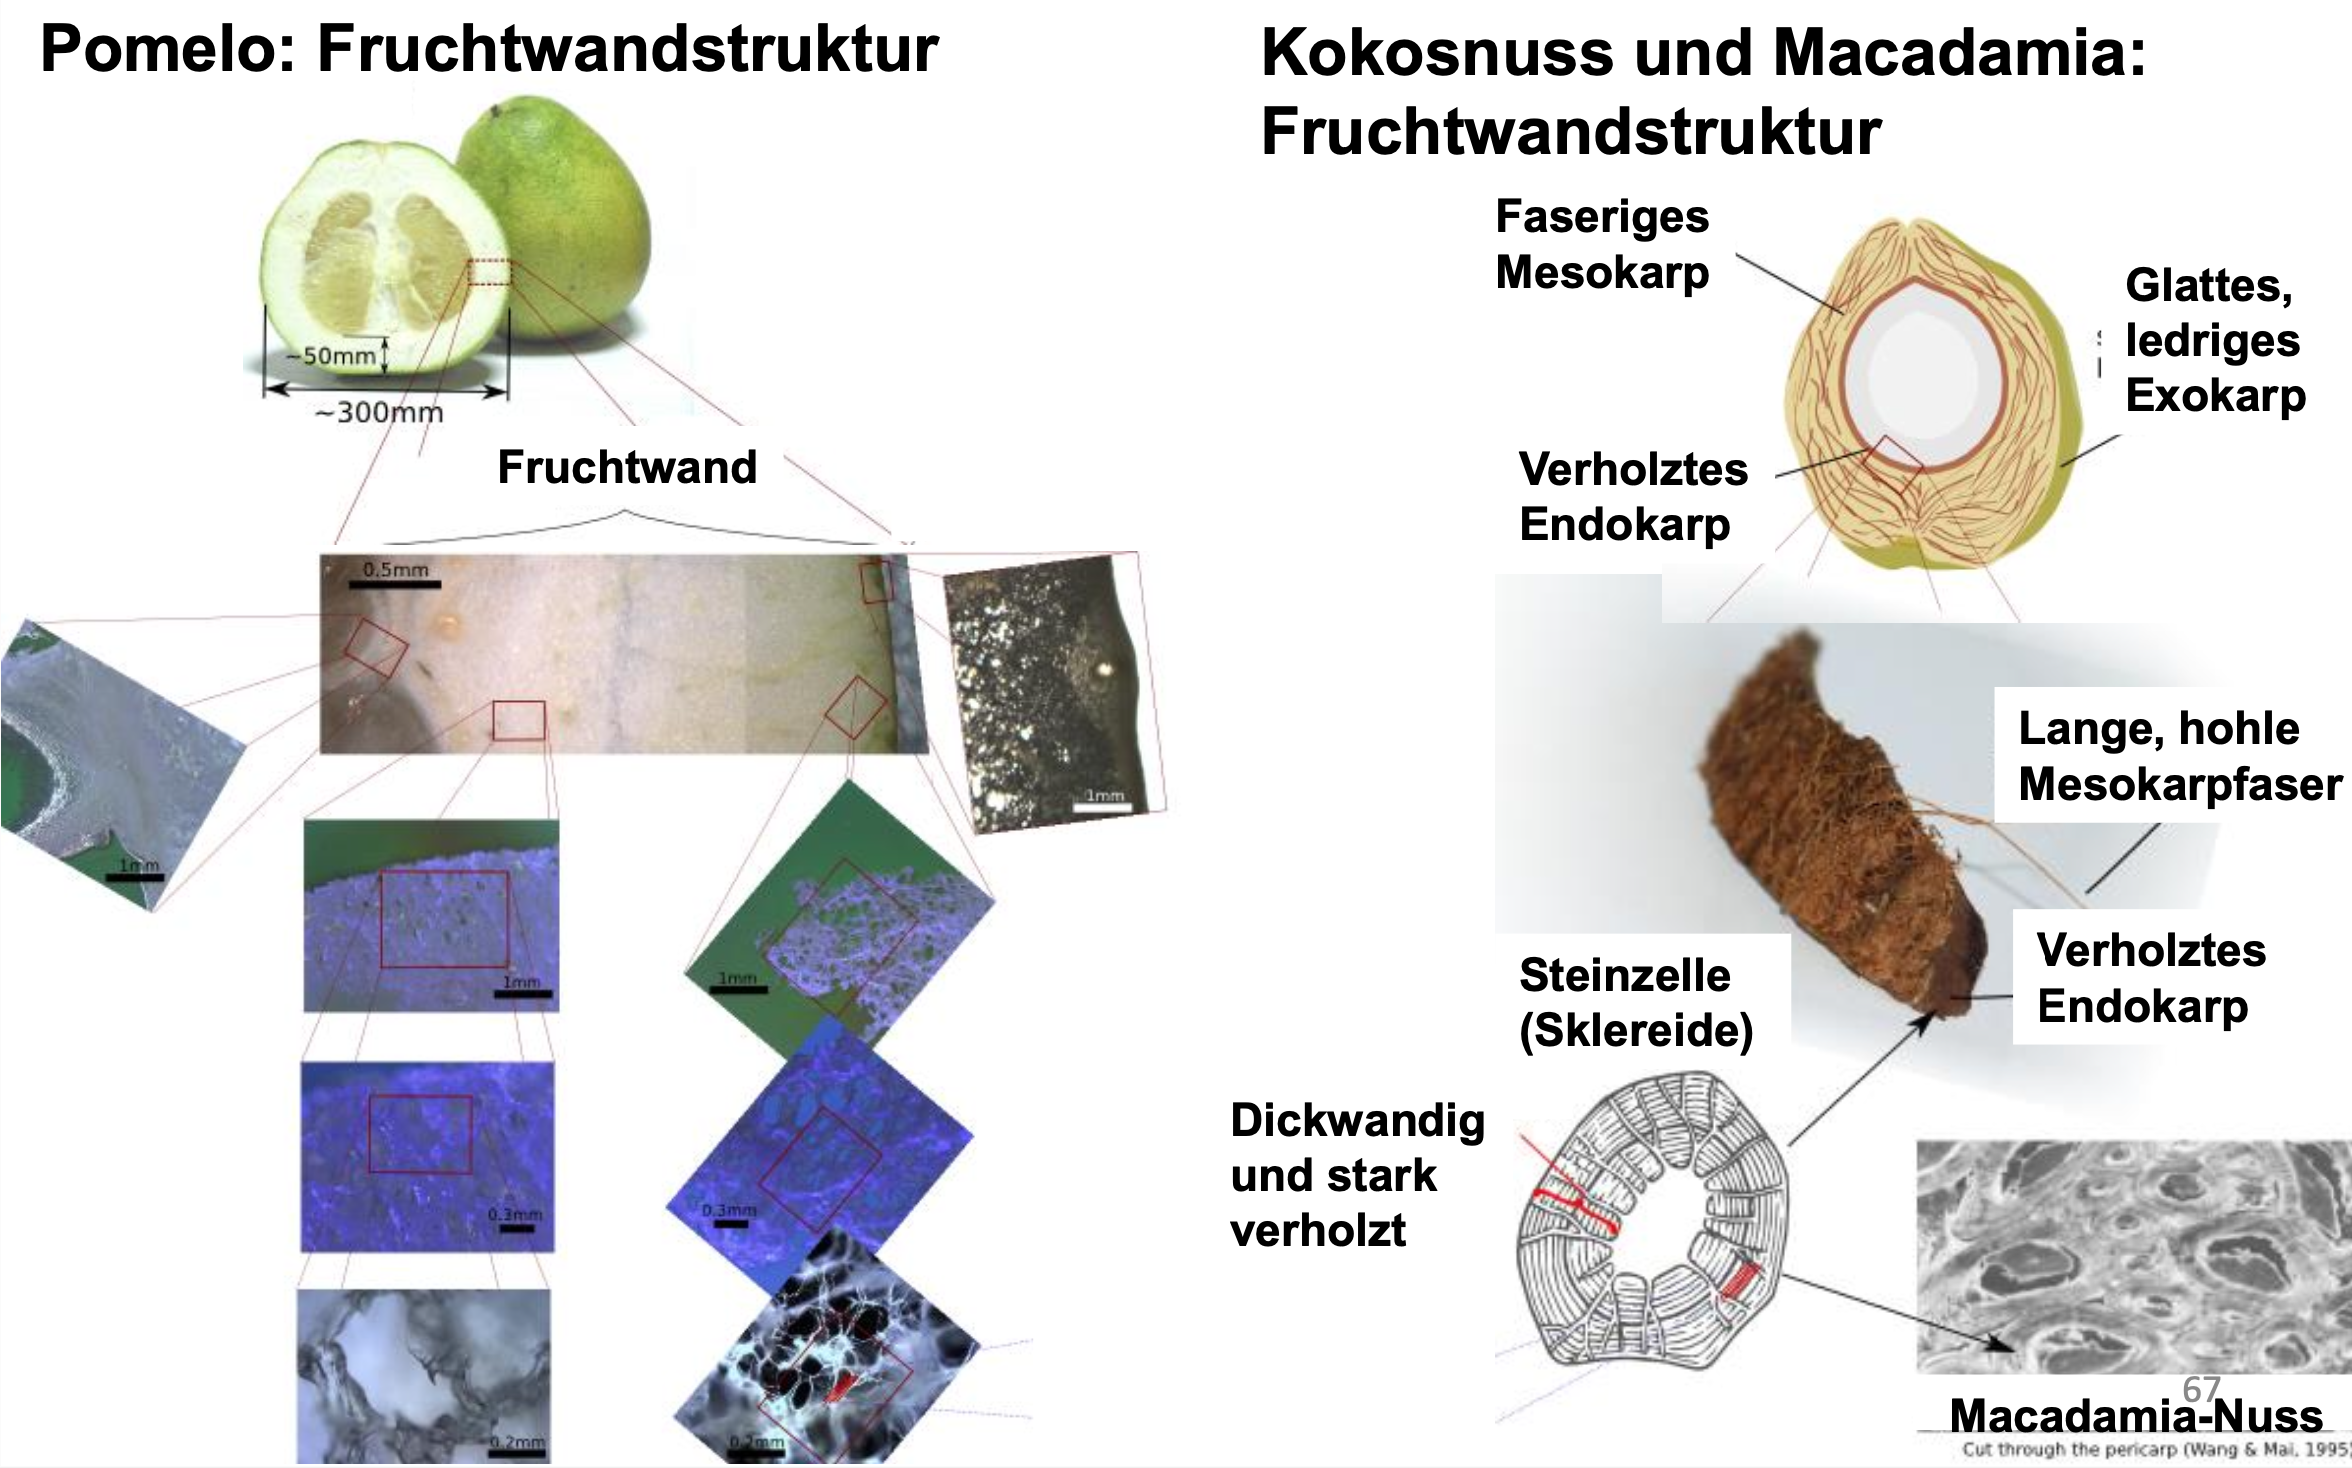
\includegraphics[width=12cm]{lec6/figures/fruchtwand.png}
\end{center}

\subsubsection{Faltstrukturen zur Verpackung auf engstem Raum}

\textbf{Blüten, Blätter, Käferflügel:} Sonnensegel für Satelliten müssen zu Beginn ihres Einsatzes ausgefaltet werden. Beispiele für Faltungen finden sich z.B.\ bei Kaktusblüten, Fangblättern von fleischfressenden Pflanzen, den Hinterflügeln des Maikäfers (technisch in Faltstühle umgesetzt \dangersign) und den Hautkragen der Kragenechse.
\\\\
\textbf{Verpackungs- \& Materialeffizienz Bienenwaben:} Direkt nach dem Bau haben die Bienenwaben eine runde Form. Durch den Flügelschlag der Bienen erwärmt sich das Wachs auf die Sprungtemperatur sodass die hexagonale Struktur entsteht
\\\\
\textbf{Bionische Kabeldurchführungen nach dem Vorbild biologischer Falt-Klapp-Strukturen:} Dabei ist es das Ziel, eine Kabeldurchführung zu entwickeln, die sowohl eine hohe Schutzklasse besitzt (dichte gegenüber Flüssigkeiten und Staub) und nicht ausgebaut werden muss, um Stecker hindurchzuführen. \textit{Hohe Öffnungs-/Schließverhältnisse} finden sich z.B.\ in den Schlauch-Muskelsystemen bei Regenwürmern, Korallentieren und Seeigeln.

\begin{center}
    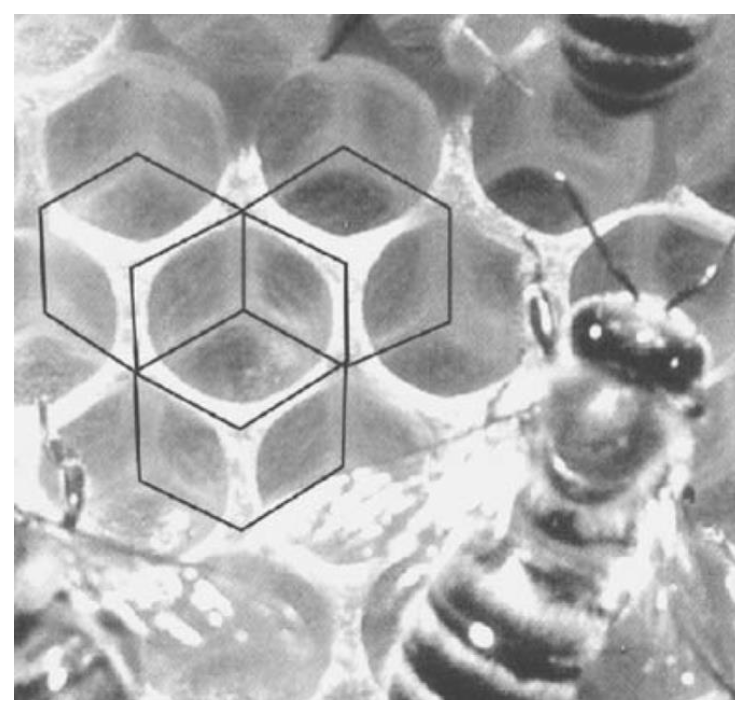
\includegraphics[width=4cm]{lec6/figures/biene.png}
    \hfill
    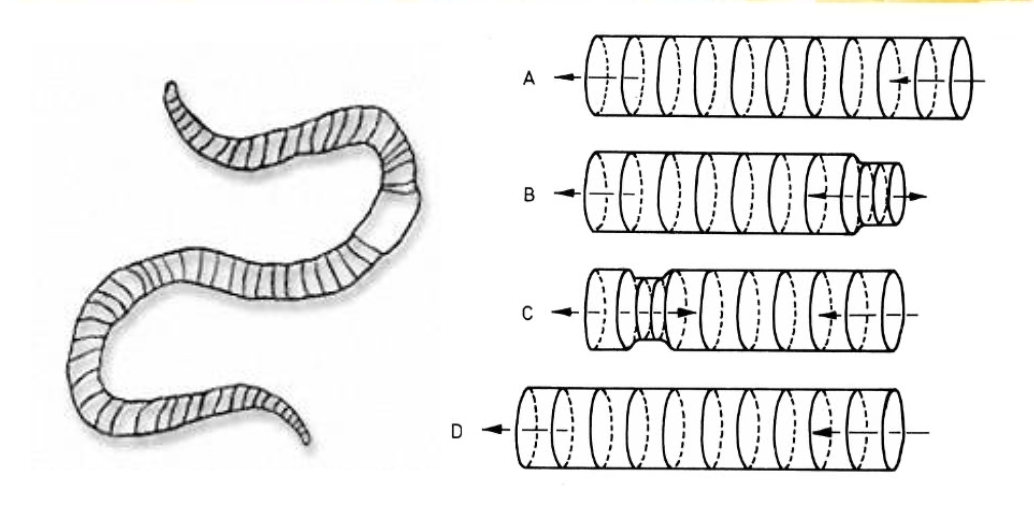
\includegraphics[width=6cm]{lec6/figures/regenwurm.png}
    \hfill
    \includegraphics[width=6cm]{lec6/figures/kabeldurchführung.png}
\end{center}
Bei Tieren sind diese Falt-/Klappstrukturen meist Muskel-gesteuert,
bei Pflanzen hingegen durch Wasserdruck gesteuert. \textit{Biologische Strukturen mit ``hoher Fähigkeit abzudichten''} sind z.B.\ Blüten. Eine Bionische Kabeldurchführung nach diesem Vorbild kann schnell öffnen und präzise schließen, dichtet gegen Staub und Spritzwasser ab, erreicht aber nicht die höchsten Schutznormen. (\dangersign $\rightarrow$ \textit{Bspl.})

\begin{center}
    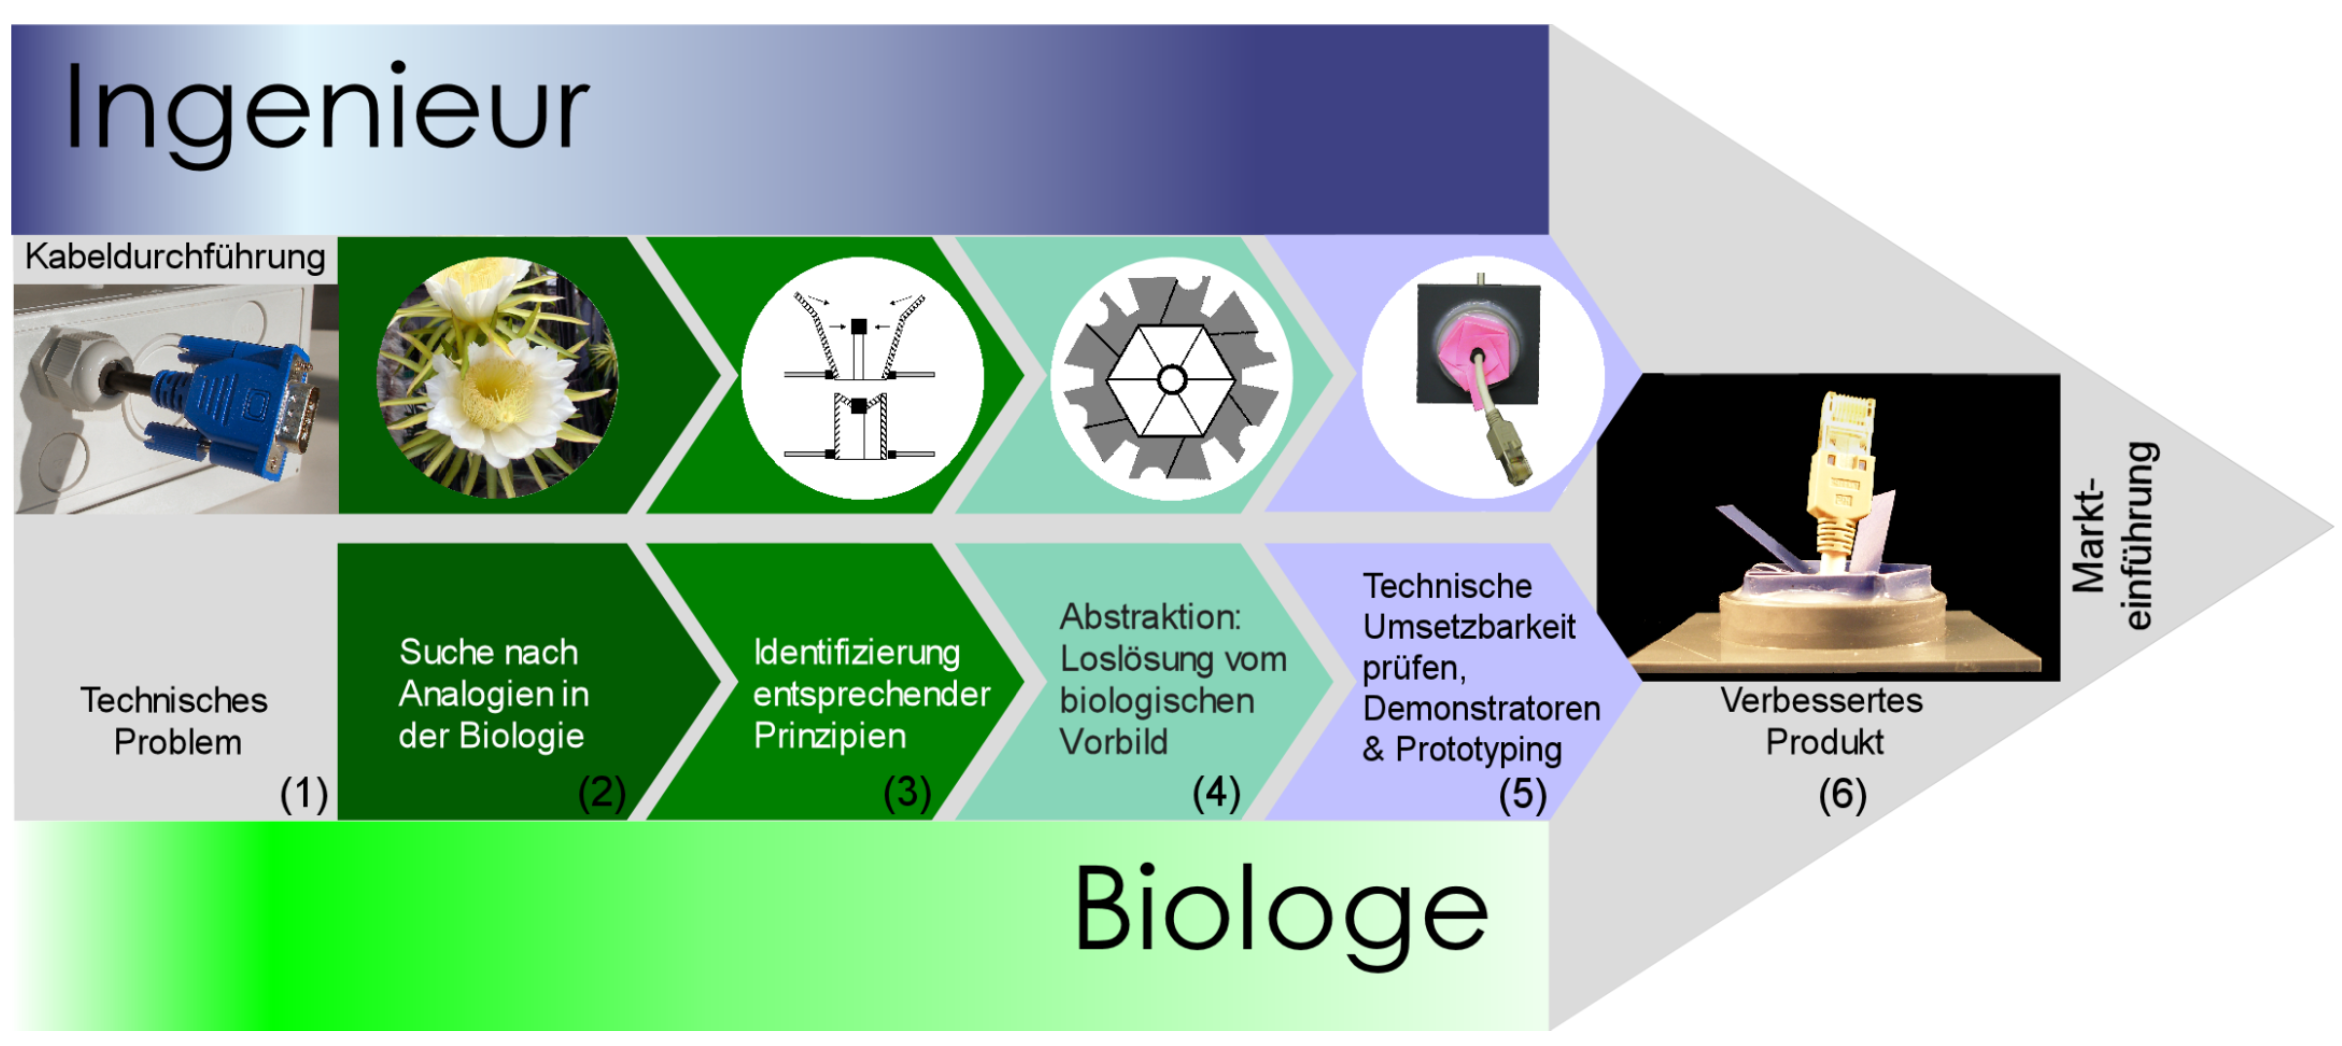
\includegraphics[width=11cm]{lec6/figures/top-down.png}
\end{center}
\textbf{Strukturoptimierte, schockabsorbierende Transportpalette aus Naturfaserverbundstoff.} Transportpaletten sind nicht mehr verwendbar, wenn z.B.\ deren Tragfähigkeit beeinträchtigt ist oder sie komtaminiert sind. Gibt es hier eine bionische Verbesserung? Die Stacheln von Igeln sind sehr stabil \& dämpfend in eine vordefinierte Biegerichtung. Deckplatten aus Naturfasern (Bäume, Bambus, etc.) sind schwer entflammbar, wasserabweisend und wiederverwertbar. In der Kombination entsteht eine Palette mit \textbf{geringerem Gewicht und modularer Dämpfung}. Probleme vor der Serienreife dieses Produkts sind allerdings hohe Herstellungskosten und die Notwendigkeit zusätzlicher Kompetenzen in der Produktion.
\\\\
(\dangersign Was ist das biologische Vorbild der bionischen Palette + Vor- \& Nachteile?)
\begin{center}
    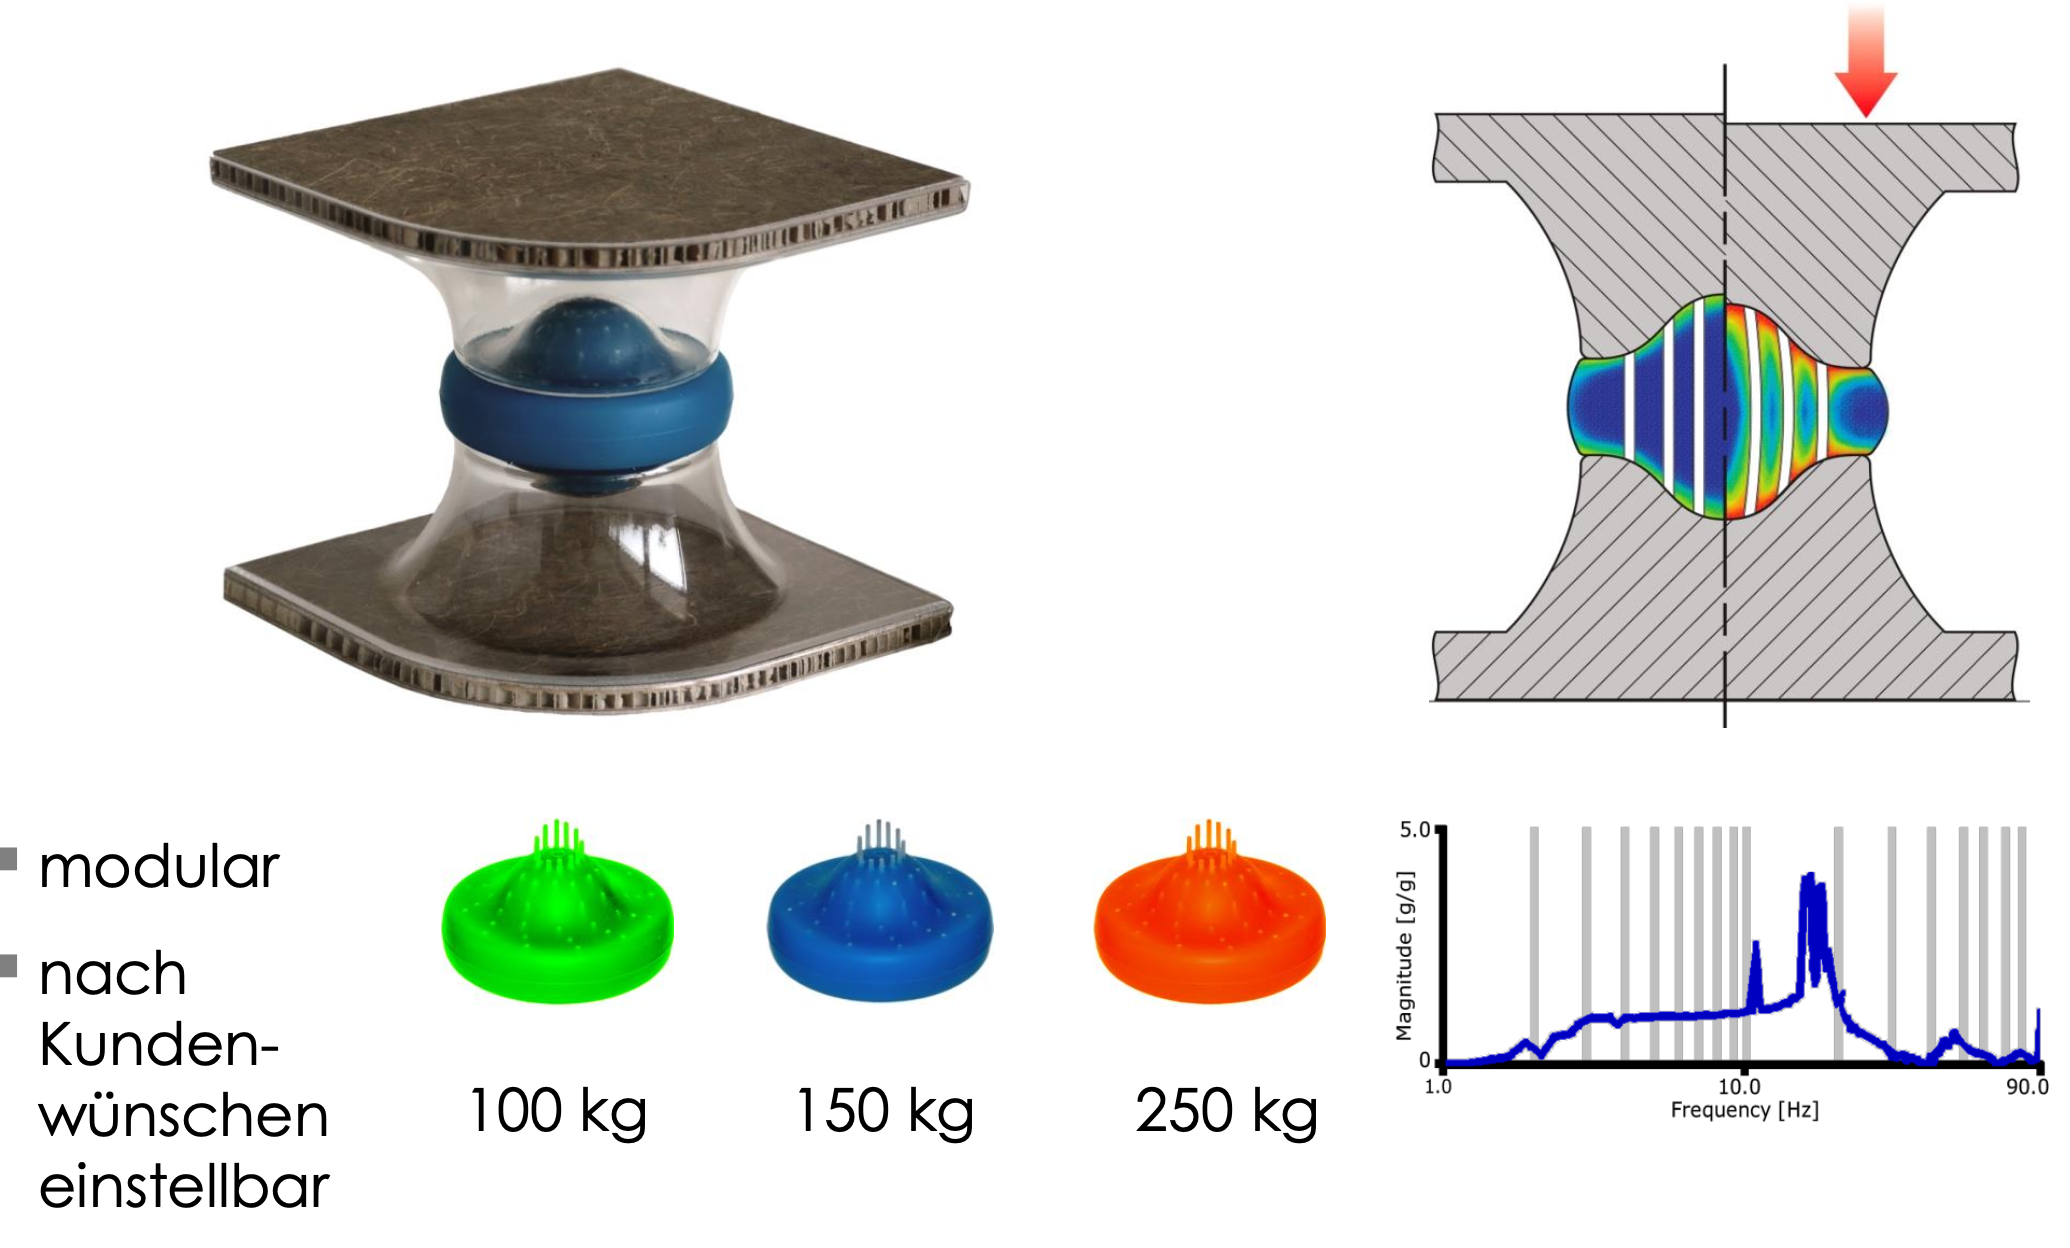
\includegraphics[width=8cm]{lec6/figures/palette.png}
    \hfill
    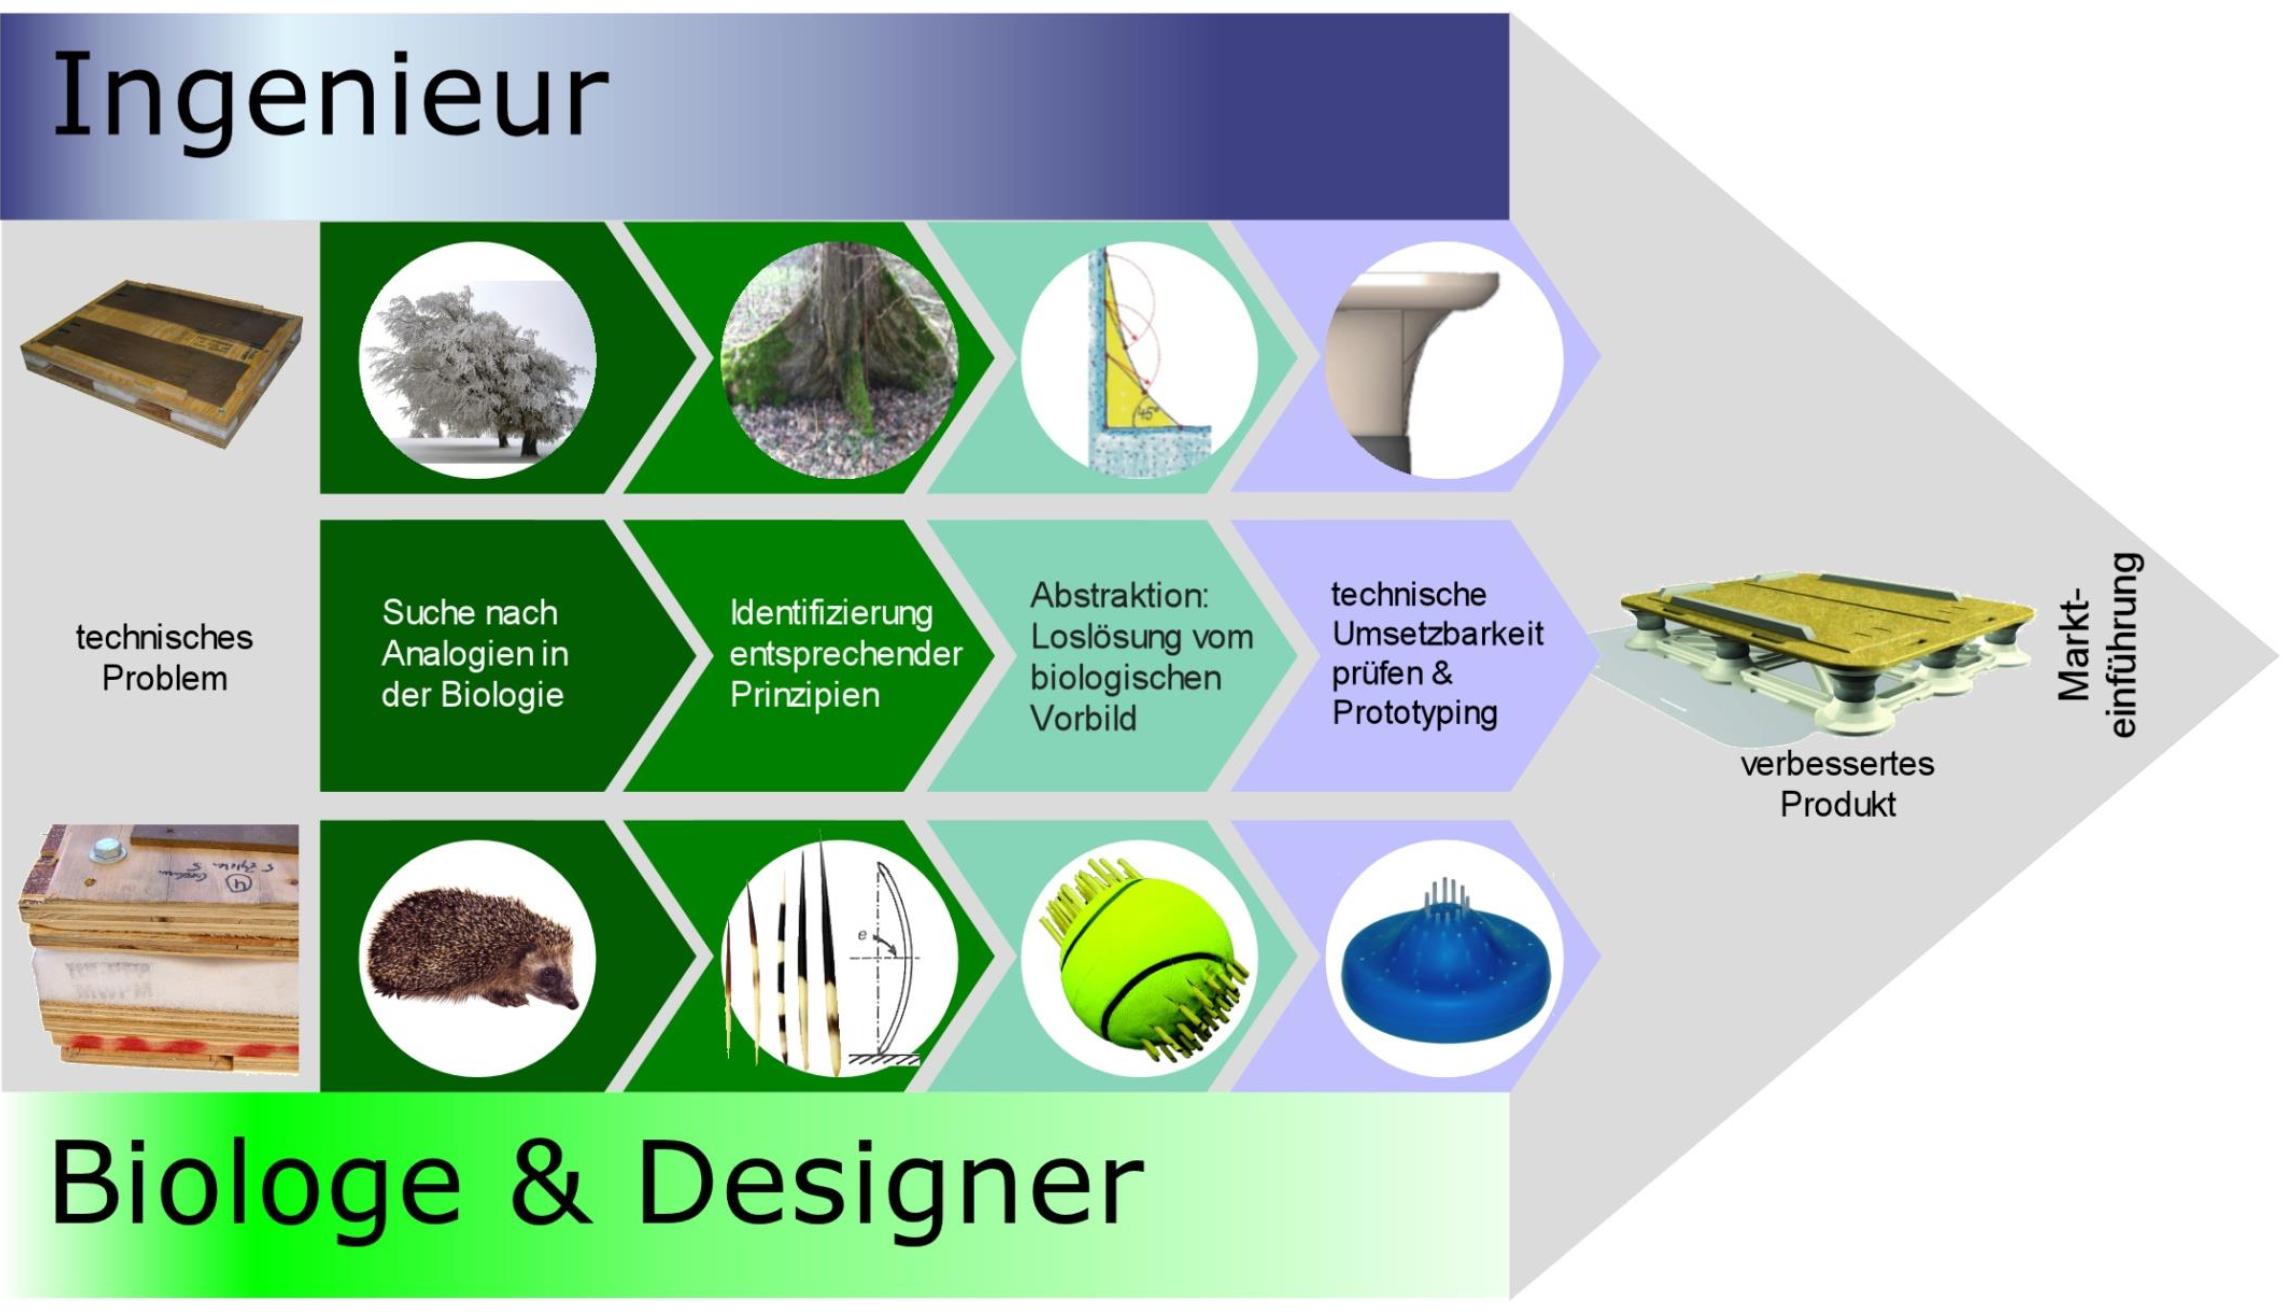
\includegraphics[width=8cm]{lec6/figures/palette-top-down.png}
\end{center}

